\documentclass[12pt,a4paper,oneside]{report}

% --- THIẾT LẬP FONT VÀ TIẾNG VIỆT CHO XELATEX ---
\usepackage{fontspec}
\setmainfont{Times New Roman}

% --- THIẾT LẬP CĂN LỀ CHUẨN KHOA CNTT - TDTU ---
% Lề trái 3.5cm, phải 2.0cm, trên 2.5cm, dưới 2.5cm
\usepackage[a4paper, left=3.5cm, right=2.0cm, top=2.5cm, bottom=2.5cm]{geometry}

% --- DÃN DÒNG VÀ ĐOẠN VĂN ---
\usepackage{setspace}
\onehalfspacing % Dãn dòng 1.5 lines
\setlength{\parindent}{1.27cm} % Thụt đầu dòng 1.27 cm (0.5 inch)
\setlength{\parskip}{4pt}      % Khoảng cách đoạn
\fontsize{13pt}{19.5pt}\selectfont % Cỡ chữ chuẩn 13pt

% --- CÁC GÓI TOÁN HỌC, ĐỒ HỌA VÀ BẢNG BIỂU ---
\usepackage{amsmath, amssymb, amsfonts}
\usepackage{graphicx}
\usepackage{float}
\usepackage{booktabs}
\usepackage{array}
\usepackage{tabularx}
\usepackage{longtable}
\usepackage{multirow}
\usepackage{caption}
\usepackage{subcaption}
\usepackage{tikz}
\usetikzlibrary{calc, arrows.meta, positioning, shapes.geometric}

% --- THUẬT TOÁN VÀ ĐOẠN MÃ NGUỒN ---
\usepackage{algorithm}
\usepackage{algorithmic}
\usepackage{listings}
\usepackage{xcolor}

\lstdefinelanguage{json}{
    basicstyle=\scriptsize\ttfamily,
    numbers=left,
    numberstyle=\tiny\color{gray},
    stepnumber=1,
    numbersep=8pt,
    showstringspaces=false,
    breaklines=true,
    frame=lines,
    backgroundcolor=\color{black!2},
    literate=
     *{0}{{{\color{blue!80!black}0}}}{1}
      {1}{{{\color{blue!80!black}1}}}{1}
      {2}{{{\color{blue!80!black}2}}}{1}
      {3}{{{\color{blue!80!black}3}}}{1}
      {4}{{{\color{blue!80!black}4}}}{1}
      {5}{{{\color{blue!80!black}5}}}{1}
      {6}{{{\color{blue!80!black}6}}}{1}
      {7}{{{\color{blue!80!black}7}}}{1}
      {8}{{{\color{blue!80!black}8}}}{1}
      {9}{{{\color{blue!80!black}9}}}{1}
      {:}{{{\color{red!80!black}:}}}{1}
      {,}{{{\color{red!80!black},}}}{1}
      {\{}{{{\color{black!80}\{}}}{1}
      {\}}{{{\color{black!80}\}}}}{1}
      {[}{{{\color{black!80}[}}}{1}
      {]}{{{\color{black!80}]}}}{1},
}

\lstset{
    basicstyle=\small\ttfamily,
    keywordstyle=\color{blue}\bfseries,
    commentstyle=\color{gray}\itshape,
    stringstyle=\color{red!70!black},
    numbers=left,
    numberstyle=\tiny\color{gray},
    stepnumber=1,
    numbersep=8pt,
    showstringspaces=false,
    breaklines=true,
    frame=lines,
    backgroundcolor=\color{black!2}
}

% --- ĐỊNH NGHĨA TIÊU ĐỀ BẢNG VÀ HÌNH CHUẨN KHOA ---
\renewcommand{\figurename}{Hình}
\renewcommand{\tablename}{Bảng}
\captionsetup[figure]{labelfont=bf, textfont=it, labelsep=colon, justification=centering}
\captionsetup[table]{labelfont=bf, textfont=it, labelsep=colon, justification=centering}

% --- CẤU HÌNH LIÊN KẾT HYPERREF ---
\usepackage[unicode, hidelinks]{hyperref}
\hypersetup{
    colorlinks=true,
    linkcolor=blue!80!black,
    citecolor=blue!80!black,
    urlcolor=blue!80!black
}

% --- ĐỊNH DẠNG TIÊU ĐỀ CHƯƠNG THEO MẪU KHOA CNTT ---
\usepackage{titlesec}
\titleformat{\chapter}[block]
  {\normalfont\Large\bfseries\centering}
  {\chaptertitlename\ \thechapter.}{0.5em}{\Large}
\titlespacing*{\chapter}{0pt}{-20pt}{20pt}

\titleformat{\section}
  {\normalfont\large\bfseries}{\thesection}{1em}{}
\titleformat{\subsection}
  {\normalfont\normalsize\bfseries}{\thesubsection}{1em}{}
\titleformat{\subsubsection}
  {\normalfont\normalsize\bfseries\itshape}{\thesubsubsection}{1em}{}

\renewcommand{\chaptername}{CHƯƠNG}
\renewcommand{\contentsname}{MỤC LỤC}
\renewcommand{\listfigurename}{DANH MỤC HÌNH VẼ}
\renewcommand{\listtablename}{DANH MỤC BẢNG BIỂU}

% ==================== NỘI DUNG TÀI LIỆU ====================
\begin{document}

% 1. TRANG BÌA NGOÀI VÀ TRANG BÌA PHỤ (KHÔNG ĐÁNH SỐ TRANG)
\pagestyle{empty}
\begin{titlepage}

\begin{tikzpicture}[remember picture, overlay]
  % Khung viền ngoài
  \draw[line width = 2pt, color = blue!80!black] 
    ($(current page.north west) + (2.5cm,-2.0cm)$) 
    rectangle 
    ($(current page.south east) + (-1.5cm,2.0cm)$);
  % Khung viền trong
  \draw[line width = 0.8pt, color = blue!80!black] 
    ($(current page.north west) + (2.6cm,-2.1cm)$) 
    rectangle 
    ($(current page.south east) + (-1.6cm,2.1cm)$);
\end{tikzpicture}

\begin{center}
    {\large \bfseries TỔNG LIÊN ĐOÀN LAO ĐỘNG VIỆT NAM}\\[0.2cm]
    {\large \bfseries TRƯỜNG ĐẠI HỌC TÔN ĐỨC THẮNG}\\[0.2cm]
    {\large \bfseries KHOA CÔNG NGHỆ THÔNG TIN}\\[1.2cm]

    
\includegraphics[width=3.5cm]{figures/image1.png}\\[1.2cm]

    {\large \bfseries NGUYỄN TẤN MẠNH – 52300221}\\[0.2cm]
    {\large \bfseries VÕ ANH KIỆT – 523H0048}\\[1.2cm]

    {\LARGE \bfseries BÁO CÁO ĐỒ ÁN CHUYÊN NGÀNH}\\[0.2cm]
    {\LARGE \bfseries CÔNG NGHỆ THÔNG TIN 2}\\[0.8cm]

    {\LARGE \bfseries HỆ THỐNG QUẢN LÝ KÝ TÚC XÁ THÔNG MINH}\\[0.3cm]
    {\LARGE \bfseries (SMARTDORM)}\\[0.4cm]
    {\large \bfseries (GIÁM SÁT VI KHÍ HẬU, AN NINH RFID, CẢNH BÁO PCCC KHẨN CẤP}\\[0.1cm]
    {\large \bfseries VÀ ĐIỀU KHIỂN THIẾT BỊ PHÒNG)}\\[1.8cm]

    {\large \bfseries THÀNH PHỐ HỒ CHÍ MINH, NĂM 2026}
\end{center}
\end{titlepage}

\begin{titlepage}

\begin{tikzpicture}[remember picture, overlay]
  % Khung viền ngoài
  \draw[line width = 2pt, color = blue!80!black] 
    ($(current page.north west) + (2.5cm,-2.0cm)$) 
    rectangle 
    ($(current page.south east) + (-1.5cm,2.0cm)$);
  % Khung viền trong
  \draw[line width = 0.8pt, color = blue!80!black] 
    ($(current page.north west) + (2.6cm,-2.1cm)$) 
    rectangle 
    ($(current page.south east) + (-1.6cm,2.1cm)$);
\end{tikzpicture}

\begin{center}
    {\large \bfseries TỔNG LIÊN ĐOÀN LAO ĐỘNG VIỆT NAM}\\[0.2cm]
    {\large \bfseries TRƯỜNG ĐẠI HỌC TÔN ĐỨC THẮNG}\\[0.2cm]
    {\large \bfseries KHOA CÔNG NGHỆ THÔNG TIN}\\[1.0cm]

    
\includegraphics[width=3.5cm]{figures/image1.png}\\[1.0cm]

    {\large \bfseries NGUYỄN TẤN MẠNH – 52300221}\\[0.2cm]
    {\large \bfseries VÕ ANH KIỆT – 523H0048}\\[1.0cm]

    {\LARGE \bfseries BÁO CÁO ĐỒ ÁN CHUYÊN NGÀNH}\\[0.2cm]
    {\LARGE \bfseries CÔNG NGHỆ THÔNG TIN 2}\\[0.8cm]

    {\LARGE \bfseries HỆ THỐNG QUẢN LÝ KÝ TÚC XÁ THÔNG MINH}\\[0.3cm]
    {\LARGE \bfseries (SMARTDORM)}\\[0.3cm]
    {\large \bfseries (GIÁM SÁT VI KHÍ HẬU, AN NINH RFID, CẢNH BÁO PCCC KHẨN CẤP}\\[0.1cm]
    {\large \bfseries VÀ ĐIỀU KHIỂN THIẾT BỊ PHÒNG)}\\[1.2cm]

    \vspace{0.5cm}
    {\large \bfseries Giảng viên hướng dẫn: TS. PHÙ TRẦN TÍN}\\[2.0cm]

    {\large \bfseries THÀNH PHỐ HỒ CHÍ MINH, NĂM 2026}
\end{center}
\end{titlepage}


% 2. PHẦN ĐẦU (ĐÁNH SỐ TRANG LA MÃ: i, ii, iii, iv, v...)
\newpage
\pagestyle{plain}
\pagenumbering{roman}

\chapter*{LỜI CẢM ƠN}
\addcontentsline{toc}{chapter}{LỜI CẢM ƠN}

Lời đầu tiên, nhóm tác giả xin được bày tỏ lòng biết ơn sâu sắc và chân thành nhất đến quý Thầy, Cô Khoa Công nghệ Thông tin – Trường Đại học Tôn Đức Thắng, những người đã tận tâm truyền đạt tri thức quý báu, phương pháp tư duy khoa học và niềm đam mê nghiên cứu công nghệ trong suốt thời gian học tập tại trường.

Đặc biệt, nhóm xin gửi lời tri ân sâu sắc nhất đến \textbf{TS. Phù Trần Tín}, người Thầy hướng dẫn đã luôn tận tình định hướng đề tài, dành nhiều thời gian trao đổi, giải đáp những vướng mắc chuyên môn sâu sắc và luôn tạo điều kiện thuận lợi nhất để nhóm hoàn thành xuất sắc đồ án \textbf{``Hệ thống Quản lý Ký túc xá Thông minh (SmartDorm)''}.

Nhóm tác giả cũng xin gửi lời cảm ơn chân thành đến Ban Quản lý Ký túc xá Trường Đại học Tôn Đức Thắng cùng các bạn sinh viên nội trú đã nhiệt tình hỗ trợ, cung cấp thông tin thực tế về quy trình vận hành phòng ở, công tác kiểm soát an ninh ra vào và các yêu cầu nghiêm ngặt về phòng cháy chữa cháy trong môi trường học đường, giúp hệ thống có tính ứng dụng cao và bám sát thực tiễn vận hành.

Cuối cùng, chúng tôi xin bày tỏ lòng biết ơn vô hạn đến gia đình, người thân và bạn bè – những người luôn là điểm tựa tinh thần vững chắc, luôn động viên, chia sẻ và đồng hành cùng nhóm trong suốt quá trình học tập và hoàn thành đồ án này.

Dù đã dành nhiều nỗ lực và thời gian nghiên cứu nghiêm túc, song do giới hạn về kinh nghiệm thực tiễn, đề tài khó tránh khỏi những thiếu sót nhất định. Nhóm kính mong nhận được những lời nhận xét, góp ý quý báu từ quý Thầy Cô trong Hội đồng phản biện để đề tài ngày càng hoàn thiện và nâng cao tính khả thi khi ứng dụng rộng rãi.

\vspace{1.5cm}
\begin{flushright}
    \textit{TP. Hồ Chí Minh, năm 2026}\\[0.3cm]
    \textbf{Nhóm sinh viên thực hiện}\\[0.2cm]
    \textit{Nguyễn Tấn Mạnh – Võ Anh Kiệt}
\end{flushright}
\newpage

\chapter*{LỜI CAM ĐOAN}
\addcontentsline{toc}{chapter}{LỜI CAM ĐOAN}

Chúng tôi xin cam đoan rằng toàn bộ nội dung trong bản báo cáo Đồ án Chuyên ngành Công nghệ Thông tin 2 với đề tài \textbf{``Hệ thống Quản lý Ký túc xá Thông minh (SmartDorm)''} là công trình nghiên cứu và thực nghiệm độc lập do chính nhóm tác giả thực hiện dưới sự hướng dẫn khoa học của \textbf{TS. Phù Trần Tín}.

Các số liệu, mã nguồn chương trình, sơ đồ nguyên lý mạch phần cứng và kết quả thực nghiệm được trình bày trong báo cáo hoàn toàn trung thực, phản ánh chính xác kết quả xây dựng, đo đạc và kiểm thử hệ thống trong thực tế. Toàn bộ các tài liệu tham khảo, thư viện mã nguồn mở và công trình liên quan đều được trích dẫn đầy đủ, rõ ràng và tuân thủ nghiêm ngặt các quy định về quyền sở hữu trí tuệ.

Nếu phát hiện có bất kỳ sự gian lận nào, chúng tôi xin hoàn toàn chịu trách nhiệm về nội dung Đồ án của mình. Trường Đại học Tôn Đức Thắng không liên quan đến những vi phạm tác quyền, bản quyền do chúng tôi gây ra trong quá trình thực hiện (nếu có).

\vspace{1.5cm}
\noindent
\begin{minipage}[t]{0.48\textwidth}
    \centering
    \textit{TP. Hồ Chí Minh, năm 2026}\\[0.2cm]
    \textbf{Tác giả}\\[0.1cm]
    
\includegraphics[height=1.8cm]{figures/signature_manh.png}\\[0.1cm]
    \textbf{Nguyễn Tấn Mạnh}\\[0.1cm]
    MSSV: 52300221
\end{minipage}
\hfill
\begin{minipage}[t]{0.48\textwidth}
    \centering
    \textit{TP. Hồ Chí Minh, năm 2026}\\[0.2cm]
    \textbf{Tác giả}\\[0.1cm]
    
\includegraphics[height=1.8cm]{figures/signature_kiet.png}\\[0.1cm]
    \textbf{Võ Anh Kiệt}\\[0.1cm]
    MSSV: 523H0048
\end{minipage}
\newpage

\chapter*{TÓM TẮT}
\addcontentsline{toc}{chapter}{TÓM TẮT}

\begin{center}
    {\large \bfseries HỆ THỐNG QUẢN LÝ KÝ TÚC XÁ THÔNG MINH (SMARTDORM)}\\[0.5cm]
\end{center}

Công tác quản lý và vận hành ký túc xá sinh viên tại các trường đại học hiện nay đang đối mặt với nhiều bài toán cấp bách, bao gồm: nguy cơ mất an toàn phòng cháy chữa cháy (chập cháy thiết bị điện, rò rỉ khí gas nguy hiểm từ khu vực sinh hoạt), quy trình kiểm soát an ninh ra vào thủ công tốn kém nhân lực và dễ xảy ra sai sót, cũng như sự thiếu vắng một nền tảng số hóa tập trung giúp sinh viên tương tác minh bạch với ban quản lý. Xuất phát từ thực tiễn đó, đề tài \textbf{``Hệ thống Quản lý Ký túc xá Thông minh (SmartDorm)''} được thiết kế và hiện thực hóa với kiến trúc 5 tầng toàn diện (Tầng thiết bị nhúng IoT, Tầng truyền thông mạng, Tầng xử lý nghiệp vụ Backend, Tầng cơ sở dữ liệu và Tầng giao diện người dùng đa nền tảng), tập trung giải quyết trọn vẹn các yêu cầu về an toàn, an ninh và tiện ích phòng ở.

Ở tầng phần cứng, hệ thống tích hợp nút mạng IoT dựa trên vi điều khiển ESP32 DevKit V1 (NodeMCU-32S) kết nối cảm biến nhiệt độ - độ ẩm kỹ thuật số DHT22, cảm biến phát hiện khí gas/khói nồng độ cao MQ-2, module relay 4 kênh cách ly quang điều khiển độc lập các phụ tải (đèn chiếu sáng, quạt thông gió, khóa cửa điện từ Solenoid), còi báo động Active Buzzer 5V và hệ thống nút bấm vật lý hỗ trợ điều khiển tại chỗ. Đặc biệt, hệ thống tích hợp cơ chế kiểm soát an ninh thẻ từ RFID (chuẩn 13.56 MHz) với thuật toán sinh mã thẻ tất định tự động theo mã số sinh viên dựa trên hàm băm SHA-256. Để đảm bảo an toàn tuyệt đối về phòng cháy chữa cháy, hệ thống xây dựng cơ chế Rule Engine tự động: ngay khi nồng độ khí gas đạt ngưỡng nguy hiểm ($\ge 80\%$), hệ thống lập tức kích hoạt còi báo động tại chỗ, tự động cắt toàn bộ relay nguồn điện của phòng để triệt tiêu nguồn phát sinh tia lửa điện, đồng thời phát lệnh cảnh báo khẩn cấp tức thời (Emergency Broadcast) đến ban quản lý qua nhiều kênh truyền thông.

Ở tầng phần mềm, hệ thống backend được xây dựng trên nền tảng NestJS (TypeScript) theo kiến trúc Clean Architecture mô-đun hóa, tích hợp giao thức truyền thông nhẹ MQTT (Eclipse Mosquitto QoS 1) với độ trễ truyền nhận dưới $40\text{ms}$, WebSockets (Socket.IO) cập nhật dữ liệu vi khí hậu và trạng thái thiết bị thời gian thực dưới $15\text{ms}$, và Prisma ORM kết nối cơ sở dữ liệu SQLite/PostgreSQL chuẩn hóa 12 thực thể. Hệ thống áp dụng mẫu thiết kế Command Pattern với cơ chế hoàn tác (Undo) cho phép khôi phục trạng thái thiết bị tức thì, cùng hệ thống thông báo đa kênh tự động gồm Telegram Bot và Email SMTP (Nodemailer). Bên cạnh đó, hệ thống tích hợp phân hệ trí tuệ nhân tạo (AI Anomaly Detection) nhằm phát hiện sớm các bất thường môi trường phòng ở và trợ lý ảo thông minh AI Copilot hỗ trợ giải thích nguyên nhân sự cố cho ban quản lý. Giao diện người dùng phát triển trên Next.js 16 với hai phân hệ phân quyền nghiêm ngặt (Admin Portal và Student Portal), hỗ trợ đầy đủ các biểu đồ thống kê và tính năng xuất báo cáo thật định dạng Excel/CSV. Kết quả kiểm thử toàn diện trên 84 ca kiểm thử tự động khẳng định tính ổn định, độ tin cậy và giá trị ứng dụng thực tiễn của đề tài.

\vspace{0.5cm}
\noindent \textbf{Từ khóa:} Smart Dormitory, Internet of Things (IoT), ESP32, PCCC tự động, RFID, Command Pattern with Undo, NestJS, Next.js, MQTT, WebSockets, Anomaly Detection.

\newpage

\chapter*{ABSTRACT}
\addcontentsline{toc}{chapter}{ABSTRACT}

\begin{center}
    {\large \bfseries SMART DORMITORY MANAGEMENT SYSTEM (SMARTDORM)}\\[0.5cm]
\end{center}

Modern university dormitory management faces pressing operational challenges, particularly fire and explosion hazards stemming from electrical faults and combustible gas leakages, inefficient manual entry-exit security monitoring, and the lack of a centralized digital communication channel between students and housing administrators. To address these critical issues, this capstone project designs and implements the \textbf{``Smart Dormitory Management System (SmartDorm)''} structured upon a robust five-tier architecture encompassing IoT Edge Sensing, Network Communication, Backend Business Logic, Relational Database Storage, and Modern Responsive Web Applications.

At the hardware layer, the edge node employs an ESP32 DevKit V1 (NodeMCU-32S) microcontroller interfaced with a DHT22 digital microclimate sensor (temperature and humidity), an MQ-2 combustible gas and smoke detector, an optocoupler-isolated 4-channel relay module controlling lighting, exhaust ventilation, and solenoid door locks, a 5V active buzzer, and tactile buttons for local manual control. Access control is powered by a 13.56 MHz RFID mechanism featuring a deterministic, automated student card identifier generation algorithm based on SHA-256 hashing. Crucially, a specialized Fire Safety Rule Engine is engineered into the system: upon detecting hazardous combustible gas concentrations ($\ge 80\%$), the node immediately sounds local alarms, executes an automated room-wide electrical power cut-off to eliminate spark ignition hazards, and broadcasts high-priority emergency alerts via bi-directional communication channels.

At the software layer, the backend is built with NestJS (TypeScript) adopting clean modular architecture, integrating lightweight MQTT messaging (Eclipse Mosquitto QoS 1) with an end-to-end latency below $40\text{ms}$, bi-directional WebSockets (Socket.IO) delivering sub-15ms real-time telemetry streaming, and Prisma ORM managing 12 relational entities. The device control subsystem incorporates the Command Design Pattern with Undo capability, supported by automated multi-channel notifications via Telegram Bot Polling and SMTP Email (Nodemailer). Furthermore, an AI Anomaly Detection service detects microclimate irregularities and a conversational AI Copilot provides contextual incident explanation. The user interface, built on Next.js 16 App Router, provides strict Role-Based Access Control (RBAC) portals for administrators and residents, complete with real-time dashboards and native Excel/CSV data exports. Comprehensive regression testing across 84 automated test cases validates the high robustness, responsiveness, and practical utility of the SmartDorm system.

\vspace{0.5cm}
\noindent \textbf{Keywords:} Smart Dormitory, Internet of Things (IoT), ESP32, Fire Safety Automation, RFID Access Control, Command Pattern, NestJS, Next.js, MQTT, WebSockets, Anomaly Detection.

\newpage


% MỤC LỤC, DANH MỤC HÌNH VẼ, DANH MỤC BẢNG BIỂU
\tableofcontents
\newpage
\addcontentsline{toc}{chapter}{DANH MỤC HÌNH VẼ}
\listoffigures
\newpage
\addcontentsline{toc}{chapter}{DANH MỤC BẢNG BIỂU}
\listoftables
\newpage

\chapter*{DANH MỤC CÁC CHỮ VIẾT TẮT}
\addcontentsline{toc}{chapter}{DANH MỤC CÁC CHỮ VIẾT TẮT}

\begin{table}[H]
\centering
\small
\begin{tabular}{|p{2.8cm}|p{5.5cm}|p{6.0cm}|}
\hline
\textbf{Ký hiệu viết tắt} & \textbf{Thuật ngữ tiếng Anh} & \textbf{Ý nghĩa tiếng Việt} \\
\hline
\textbf{ADC} & Analog-to-Digital Converter & Bộ chuyển đổi tín hiệu tương tự sang số \\
\hline
\textbf{API} & Application Programming Interface & Giao diện lập trình ứng dụng \\
\hline
\textbf{CPU} & Central Processing Unit & Bộ vi xử lý trung tâm \\
\hline
\textbf{CSS} & Cascading Style Sheets & Ngôn ngữ định kiểu giao diện trang web \\
\hline
\textbf{DHT} & Digital Humidity and Temperature & Cảm biến đo nhiệt độ và độ ẩm kỹ thuật số \\
\hline
\textbf{ERD} & Entity-Relationship Diagram & Sơ đồ mối quan hệ giữa các thực thể \\
\hline
\textbf{ESP32} & Espressif Systems 32-bit SoC & Vi điều khiển tích hợp Wi-Fi và Bluetooth \\
\hline
\textbf{GPIO} & General Purpose Input/Output & Chân vào/ra mục đích chung của vi điều khiển \\
\hline
\textbf{IoT} & Internet of Things & Mạng lưới vạn vật kết nối Internet \\
\hline
\textbf{JSON} & JavaScript Object Notation & Định dạng trao đổi dữ liệu tiêu chuẩn \\
\hline
\textbf{JWT} & JSON Web Token & Chuẩn truyền tải thông tin bảo mật JSON \\
\hline
\textbf{LLM} & Large Language Model & Mô hình ngôn ngữ lớn (Trí tuệ nhân tạo) \\
\hline
\textbf{MQTT} & Message Queuing Telemetry Transport & Giao thức truyền tin thu thập số liệu nhẹ \\
\hline
\textbf{ORM} & Object-Relational Mapping & Ánh xạ đối tượng vào cơ sở dữ liệu quan hệ \\
\hline
\textbf{PCCC} & Phòng cháy chữa cháy & Công tác phòng ngừa và ứng phó sự cố cháy \\
\hline
\textbf{QoS} & Quality of Service & Mức chất lượng dịch vụ truyền tải dữ liệu \\
\hline
\textbf{RAM} & Random Access Memory & Bộ nhớ truy xuất ngẫu nhiên \\
\hline
\textbf{RBAC} & Role-Based Access Control & Kiểm soát truy cập dựa trên vai trò \\
\hline
\textbf{REST} & Representational State Transfer & Kiểu kiến trúc phần mềm cho dịch vụ web \\
\hline
\textbf{RFID} & Radio-Frequency Identification & Nhận dạng đối tượng bằng tần số vô tuyến \\
\hline
\textbf{SHA-256} & Secure Hash Algorithm 256-bit & Thuật toán băm bảo mật tiêu chuẩn an ninh \\
\hline
\textbf{SMTP} & Simple Mail Transfer Protocol & Giao thức truyền tải thư điện tử đơn giản \\
\hline
\textbf{SPI} & Serial Peripheral Interface & Chuẩn giao tiếp nối tiếp đồng bộ ngoại vi \\
\hline
\textbf{UID} & Unique Identifier & Mã định danh duy nhất của thẻ từ RFID \\
\hline
\textbf{UI/UX} & User Interface / User Experience & Giao diện người dùng / Trải nghiệm người dùng \\
\hline
\textbf{Wokwi} & Wokwi Embedded Simulator & Nền tảng mô phỏng mạch điện tử trực tuyến \\
\hline
\end{tabular}
\end{table}
\newpage


% 3. CÁC CHƯƠNG NỘI DUNG CHÍNH (ĐÁNH SỐ Ả RẬP: 1, 2, 3...)
\newpage
\pagenumbering{arabic}

\chapter{TỔNG QUAN DỰ ÁN VÀ PHÂN TÍCH YÊU CẦU}
\label{ch:chuong1}

\section{Giới thiệu và bối cảnh đề tài}
\label{sec:gioi_thieu}

Trong bối cảnh chuyển đổi số giáo dục đại học và phát triển các mô hình khuôn viên thông minh (Smart Campus), hệ thống ký túc xá (KTX) sinh viên giữ vai trò là hạ tầng sinh hoạt và học tập thiết yếu phục vụ hàng ngàn sinh viên nội trú. Một môi trường nội trú an toàn, văn minh và tiện nghi không chỉ bảo đảm sức khỏe, tính mạng cho sinh viên mà còn nâng cao hiệu quả quản lý cơ sở vật chất của nhà trường.

Tuy nhiên, qua khảo sát thực tế quy trình vận hành tại các ký túc xá sinh viên hiện nay, công tác quản trị vẫn bộc lộ nhiều điểm bất cập và rủi ro nghiêm trọng:
\begin{itemize}
    \item \textbf{Hiểm họa cháy nổ và mất an toàn phòng cháy chữa cháy (PCCC):} Nguy cơ hỏa hoạn do sự cố rò rỉ khí gas tại khu vực nấu ăn hoặc chập điện các thiết bị sinh hoạt công suất cao là mối đe dọa thường trực. Hầu hết các ký túc xá hiện nay chỉ trang bị chuông báo độc lập tại chỗ hoặc dựa vào tuần tra thủ công, thiếu cơ chế phát hiện sớm nồng độ khí gas nguy hiểm, không có khả năng tự động ngắt nguồn điện phòng để triệt tiêu nguồn phát tia lửa điện, và không thể gửi cảnh báo khẩn cấp tức thời đến ban quản lý.
    \item \textbf{Kiểm soát an ninh ra vào thủ công và thiếu chính xác:} Việc quản lý sinh viên ra vào phòng phần lớn vẫn dựa vào chìa khóa cơ truyền thống hoặc sổ sách trực ban. Chìa khóa cơ dễ bị sao chép trái phép, dễ thất lạc, gây khó khăn cho việc quản lý giờ giấc và không thể truy vết khi xảy ra sự cố mất cắp tài sản.
    \item \textbf{Thiếu vắng nền tảng số hóa quản trị tập trung:} Chưa có một hệ sinh thái phần mềm kết nối trực tiếp giữa ban quản lý và sinh viên. Khi xảy ra sự cố phòng ở, sinh viên phải báo cáo trực tiếp bằng giấy tờ hoặc liên hệ thủ công, dẫn đến độ trễ xử lý cao, thiếu dữ liệu lịch sử để thống kê và tối ưu hóa vận hành.
\end{itemize}

Nhằm giải quyết triệt để các bài toán thực tiễn nêu trên, đề tài \textbf{``Hệ thống Quản lý Ký túc xá Thông minh (SmartDorm)''} được nghiên cứu và xây dựng toàn diện, kết hợp chặt chẽ giữa phần cứng nhúng Internet of Things (IoT), hệ thống máy chủ backend xử lý thời gian thực, cơ sở dữ liệu quan hệ, phân tích trí tuệ nhân tạo (AI Anomaly Detection \& Trợ lý ảo Copilot) và giao diện web hiện đại phân quyền theo vai trò.

\section{Phân tích yêu cầu hệ thống}
\label{sec:phan_tich_yeu_cau}

\subsection{Yêu cầu chức năng}
\label{subsec:yeu_cau_chuc_nang}

Hệ thống SmartDorm phải đáp ứng đầy đủ các nhóm chức năng nghiệp vụ cốt lõi sau:
\begin{enumerate}
    \item \textbf{Giám sát môi trường và vi khí hậu phòng ở:}
    \begin{itemize}
        \item Thu thập liên tục các chỉ số nhiệt độ ($^\circ\text{C}$) và độ ẩm (\%) không khí phòng ở thông qua cảm biến kỹ thuật số DHT22 với chu kỳ từ 3 đến 5 giây.
        \item Cập nhật dữ liệu tức thời lên bảng điều khiển thời gian thực (Real-time Dashboard) mà không yêu cầu người dùng phải tải lại trang.
    \end{itemize}
    \item \textbf{Giám sát an toàn PCCC và phản ứng khẩn cấp tự động:}
    \begin{itemize}
        \item Đo lường liên tục nồng độ khí gas và khói thông qua cảm biến chuyên dụng MQ-2.
        \item Tích hợp bộ quy tắc xử lý an toàn (Rule Engine): Khi nồng độ khí gas đạt ngưỡng cảnh báo ($\ge 50\%$) hoặc nhiệt độ bất thường ($> 45^\circ\text{C}$), kích hoạt còi buzzer bíp ngắt quãng và gửi cảnh báo mức WARNING.
        \item Khi nồng độ khí gas đạt ngưỡng nguy hiểm cháy nổ ($\ge 80\%$ hoặc sự cố FIRE): Ngay lập tức kích hoạt còi hú liên tục, \textbf{tự động ngắt toàn bộ relay điện phòng} nhằm triệt tiêu tia lửa điện, đồng thời phát lệnh khẩn cấp (Emergency Broadcast) gửi thông báo đa kênh qua Telegram Bot, Email SMTP và pop-up cảnh báo đỏ trên Web.
    \end{itemize}
    \item \textbf{Kiểm soát an ninh ra vào bằng thẻ từ RFID và thuật toán tự động:}
    \begin{itemize}
        \item Quản lý lượt ra vào phòng ở thông qua công nghệ thẻ từ RFID chuẩn 13.56 MHz (RC522).
        \item Ứng dụng thuật toán sinh mã thẻ tự động dựa trên hàm băm SHA-256 kết hợp mã số sinh viên (MSSV) để cấp phát mã thẻ chuẩn định dạng \texttt{CARD\_XXXXXXXX}.
        \item Tự động đối soát UID thẻ với danh sách sinh viên nội trú của phòng: Nếu hợp lệ (\texttt{GRANTED}), kích hoạt mở khóa cửa Solenoid trong 4 giây và còi bíp xác nhận; nếu không hợp lệ (\texttt{DENIED}), giữ khóa cửa, phát 3 tiếng còi cảnh báo và ghi nhận vi phạm an ninh lên hệ thống.
    \end{itemize}
    \item \textbf{Điều khiển thiết bị phòng ở và cơ chế hoàn tác lệnh (Undo):}
    \begin{itemize}
        \item Điều khiển bật/tắt an toàn các tải thiết bị phòng: Đèn chiếu sáng, Quạt thông gió và Khóa cửa điện từ thông qua module relay cách ly quang và các nút bấm vật lý trên bo mạch.
        \item Áp dụng mẫu thiết kế Command Pattern ghi nhận lịch sử mọi thao tác điều khiển (ai thực hiện, thời gian nào, qua web hay nút bấm), cung cấp tính năng Hoàn tác lệnh gần nhất (Undo) để khôi phục trạng thái thiết bị tức thời.
    \end{itemize}
    \item \textbf{Phân tích thông minh AI và Trợ lý ảo AI Copilot:}
    \begin{itemize}
        \item Phát hiện bất thường môi trường (AI Anomaly Detection) dựa trên thuật toán Isolation Forest nhận diện các chuỗi gia tăng nhiệt độ hoặc khí gas bất thường.
        \item Tích hợp trợ lý ảo AI Copilot hỗ trợ giải thích ngữ cảnh sự cố, đề xuất phương án xử lý theo quy chuẩn an toàn và hỏi đáp dữ liệu phòng ở thời gian thực.
    \end{itemize}
    \item \textbf{Báo cáo thống kê và xuất dữ liệu thật:}
    \begin{itemize}
        \item Xuất dữ liệu báo cáo chuyên sâu định dạng Excel và CSV phục vụ công tác thanh tra và lưu trữ: Báo cáo vi khí hậu môi trường, Báo cáo kiểm soát an ninh ra vào RFID, Báo cáo sự cố khẩn cấp PCCC và Báo cáo nhật ký thiết bị.
    \end{itemize}
\end{enumerate}

\subsection{Yêu cầu an toàn và bảo mật}
\label{subsec:yeu_cau_bao_mat}

\begin{itemize}
    \item \textbf{Phân quyền truy cập dựa trên vai trò (RBAC):} Phân tách quyền hạn rõ rệt giữa hai phân hệ Quản trị viên (Admin Portal) và Sinh viên nội trú (Student Portal). Sinh viên chỉ có quyền truy cập dữ liệu và điều khiển thiết bị thuộc phòng ở của mình.
    \item \textbf{Bảo mật phiên làm việc và API:} Mọi giao tiếp giữa trình duyệt web và máy chủ backend đều được xác thực thông qua JSON Web Token (JWT) với mã hóa mật khẩu an toàn theo giải thuật băm Bcrypt Salt.
    \item \textbf{An toàn điện học đường tuyệt đối:} Phần cứng thử nghiệm tuân thủ quy chuẩn điện hạ áp, sử dụng nguồn 5V DC/3.3V DC an toàn qua cổng Type-C, loại bỏ hoàn toàn việc can thiệp trực tiếp vào điện lưới cao áp 220V nguy hiểm.
    \item \textbf{Ngăn chặn truy cập trái phép phần cứng:} Module mạng IoT ESP32 kết nối MQTT Broker qua kênh xác thực người dùng và mật khẩu riêng biệt.
\end{itemize}

\subsection{Yêu cầu phi chức năng và hiệu năng}
\label{subsec:yeu_cau_hieu_nang}

\begin{itemize}
    \item \textbf{Độ trễ truyền nhận vi điều khiển (MQTT Latency):} Thời gian từ khi cảm biến phần cứng phát tín hiệu đến khi máy chủ Backend nhận và xử lý gói tin qua MQTT Broker không vượt quá $50\text{ ms}$ (thực tế đo đạc đạt dưới $40\text{ ms}$).
    \item \textbf{Độ trễ truyền phát thời gian thực (WebSocket Latency):} Thời gian cập nhật trạng thái từ backend lên giao diện trình duyệt web qua Socket.IO đạt dưới $15\text{ ms}$.
    \item \textbf{Thời gian phản ứng ngắt điện PCCC khẩn cấp:} Từ thời điểm nồng độ khí gas vượt ngưỡng nguy hiểm $\ge 80\%$, toàn bộ quy trình gồm: hú còi tại chỗ, ngắt relay điện phòng, cập nhật trạng thái lên cơ sở dữ liệu và gửi thông báo Telegram phải hoàn tất trong vòng dưới $1.5\text{ giây}$.
    \item \textbf{Khả năng chịu tải đồng thời:} Hệ thống duy trì hoạt động ổn định khi phục vụ đồng thời 500 kết nối WebSockets và 100 yêu cầu truy vấn API mỗi giây mà không bị nghẽn đường truyền.
\end{itemize}

\section{Thiết kế hệ thống tổng thể}
\label{sec:thiet_ke_tong_the}

Hệ thống SmartDorm được tổ chức theo kiến trúc phân tầng 5 lớp (5-Tier Architecture), bảo đảm tính tách biệt độc lập giữa các thành phần, dễ dàng bảo trì và mở rộng linh hoạt:

\begin{figure}[H]
\centering
\begin{tikzpicture}[
    layer/.style={rectangle, draw=blue!80!black, fill=blue!5, thick, minimum width=14.5cm, minimum height=1.2cm, rounded corners=4pt, align=center, font=\small},
    arr/.style={-{Stealth[length=3mm]}, thick, color=blue!80!black}
]
    % Tầng 1
    \node[layer] (layer1) at (0, 0) {\textbf{TẦNG 1: THIẾT BỊ NHÚNG VÀ CẢM BIẾN IOT (EDGE HARDWARE)}\\ESP32 NodeMCU-32S, DHT22 (Nhiệt/Ẩm), MQ-2 (Gas/Khói), RFID-RC522 (13.56MHz), Relay 4 kênh, Buzzer 5V, Nút nhấn};
    
    % Tầng 2
    \node[layer] (layer2) at (0, 2.0) {\textbf{TẦNG 2: MẠNG VÀ TRUYỀN THÔNG DỮ LIỆU (NETWORK / COMMUNICATION)}\\Giao thức MQTT (Mosquitto Broker QoS 1, Port 1883) \& WebSockets (Socket.IO Real-time Engine)};
    
    % Tầng 3
    \node[layer] (layer3) at (0, 4.0) {\textbf{TẦNG 3: XỬ LÝ NGHIỆP VỤ BACKEND VÀ TRÍ TUỆ NHÂN TẠO (BACKEND SERVICES)}\\NestJS TypeScript Clean Architecture, Command Pattern with Undo, PCCC Rule Engine, Isolation Forest Anomaly Detection, AI Copilot};
    
    % Tầng 4
    \node[layer] (layer4) at (0, 6.0) {\textbf{TẦNG 4: LƯU TRỮ VÀ CƠ SỞ DỮ LIỆU (PERSISTENCE LAYER)}\\Prisma ORM, SQLite / PostgreSQL chuẩn hóa 12 thực thể quan hệ, Lịch sử lệnh, Nhật ký ra vào, Lịch sử PCCC};
    
    % Tầng 5
    \node[layer] (layer5) at (0, 8.0) {\textbf{TẦNG 5: ỨNG DỤNG VÀ TRỰC QUAN HÓA (PRESENTATION / APPLICATION)}\\Next.js 16 App Router: Admin Portal (10 phân hệ giám sát) \& Student Portal (5 phân hệ cá nhân), Xuất báo cáo Excel/CSV};

    % Mũi tên kết nối 2 chiều
    \draw[arr, <->] (layer1) -- (layer2);
    \draw[arr, <->] (layer2) -- (layer3);
    \draw[arr, <->] (layer3) -- (layer4);
    \draw[arr, <->] (layer3) -- (layer5);
\end{tikzpicture}
\caption{Sơ đồ kiến trúc 5 tầng của Hệ thống Quản lý Ký túc xá Thông minh (SmartDorm)}
\label{fig:kien_truc_5_tang}
\end{figure}

Các tầng trong kiến trúc hoạt động phối hợp nhịp nhàng:
\begin{enumerate}
    \item \textbf{Tầng 1 (Edge Hardware):} Thu thập dữ liệu cảm biến vật lý tại từng phòng KTX và điều khiển trực tiếp các tải điện thông qua module relay cách ly quang.
    \item \textbf{Tầng 2 (Communication):} Truyền dẫn dữ liệu nhẹ, tin cậy qua MQTT Broker theo chuẩn QoS 1 và đẩy dữ liệu tức thì lên máy khách qua WebSockets.
    \item \textbf{Tầng 3 (Backend Services):} Trung tâm điều phối toàn bộ luồng nghiệp vụ hệ thống, thực thi xác thực JWT, phân quyền RBAC, kiểm tra điều kiện an toàn PCCC, quản lý hàng đợi hoàn tác lệnh (Undo), và chạy các mô hình AI phát hiện bất thường môi trường.
    \item \textbf{Tầng 4 (Persistence):} Quản lý dữ liệu quan hệ qua Prisma ORM, lưu trữ có cấu trúc nhật ký ra vào, trạng thái thiết bị và các sự cố khẩn cấp.
    \item \textbf{Tầng 5 (Presentation):} Cung cấp trải nghiệm người dùng hiện đại, trực quan, hỗ trợ tương tác trên cả máy tính và thiết bị di động cho ban quản lý và sinh viên.
\end{enumerate}

\section{Công cụ và môi trường triển khai}
\label{sec:cong_cu_moi_truong}

Toàn bộ quá trình nghiên cứu, thiết kế, hiện thực và kiểm nghiệm hệ thống SmartDorm được xây dựng trên nền tảng các công cụ và công nghệ mã nguồn mở tiên tiến nhất. Bảng \ref{tab:cong_cu_trien_khai} tổng hợp danh mục công cụ phần cứng và phần mềm được sử dụng trong dự án.

\begin{table}[H]
\centering
\small
\begin{tabularx}{\textwidth}{|c|p{3.2cm}|p{2.4cm}|X|}
\hline
\textbf{STT} & \textbf{Tên công cụ / Phần mềm} & \textbf{Phiên bản} & \textbf{Vai trò và chức năng sử dụng} \\
\hline
1 & ESP32 NodeMCU-32S & CP2102 Type-C & Vi điều khiển trung tâm nút mạng IoT tại phòng KTX \\
\hline
2 & Cảm biến DHT22 & 3 chân & Đo nhiệt độ (-40 đến 80$^\circ\text{C}$) và độ ẩm (0 đến 100\%) \\
\hline
3 & Cảm biến MQ-2 & 4 chân & Phát hiện nồng độ khí gas dễ cháy (LPG, Propane) và khói \\
\hline
4 & Module Relay 4 kênh & 5V cách ly quang & Đóng/ngắt an toàn phụ tải chiếu sáng, quạt và khóa cửa \\
\hline
5 & Còi Active Buzzer & 5V DC & Phát âm thanh cảnh báo tại chỗ khi có sự cố cháy hoặc thẻ lạ \\
\hline
6 & Nút nhấn 4 chân & Tactile Button & Điều khiển bật/tắt thiết bị tại chỗ và mô phỏng quẹt thẻ RFID \\
\hline
7 & Wokwi Embedded Simulator & Online 2026 & Môi trường mô phỏng sơ đồ mạch và kiểm thử firmware nhúng \\
\hline
8 & PlatformIO / VS Code & Core 6.x & Môi trường biên dịch và nạp firmware C++ cho vi điều khiển \\
\hline
9 & NestJS Framework & v10.x & Nền tảng xây dựng máy chủ backend TypeScript Clean Architecture \\
\hline
10 & Next.js App Router & v16.x & Nền tảng xây dựng giao diện ứng dụng web Admin và Student \\
\hline
11 & Prisma ORM & v5.x & Ánh xạ đối tượng và thao tác cơ sở dữ liệu quan hệ \\
\hline
12 & Eclipse Mosquitto & v2.0.x & MQTT Message Broker trung gian điều phối bản tin IoT \\
\hline
13 & Socket.IO & v4.x & Động cơ WebSockets phát sóng dữ liệu vi khí hậu thời gian thực \\
\hline
14 & Scikit-Learn / Python & v1.4.x & Huấn luyện và vận hành mô hình Isolation Forest phát hiện bất thường \\
\hline
15 & Telegram Bot API & BotFather 2026 & Kênh gửi thông báo khẩn cấp PCCC có nút tương tác xác nhận \\
\hline
16 & Nodemailer SMTP & v6.9.x & Dịch vụ gửi thư điện tử cảnh báo khẩn cấp định dạng HTML \\
\hline
\end{tabularx}
\caption{Danh sách công cụ, phần mềm và môi trường triển khai hệ thống}
\label{tab:cong_cu_trien_khai}
\end{table}

\newpage

\chapter{THIẾT KẾ PHẦN CỨNG VÀ TRUYỀN THÔNG IOT}
\label{ch:chuong2}

\section{Sơ đồ mạch mô phỏng Wokwi chuẩn hệ thống}
\label{sec:so_do_mach_wokwi}

Để bảo đảm tính đúng đắn về nguyên lý điện tử và hạn chế tối đa rủi ro chập cháy trước khi triển khai trên linh kiện thật, toàn bộ hệ thống phần cứng IoT của SmartDorm đã được thiết kế và kiểm thử thành công trên nền tảng mô phỏng nhúng trực tuyến Wokwi. 

Hình \ref{fig:so_do_wokwi} thể hiện sơ đồ mạch điện tử hoàn chỉnh được xuất trực tiếp từ dự án mô phỏng Wokwi của hệ thống.

\begin{figure}[H]
\centering
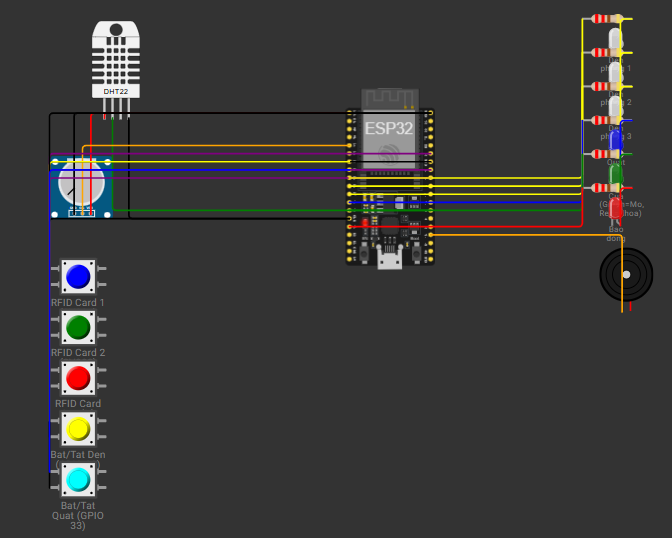
\includegraphics[width=0.95\textwidth]{figures/so_do_mach_mo_phong_wokwi.png}
\caption{Sơ đồ mạch mô phỏng hoàn chỉnh của nút mạng SmartDorm trên nền tảng Wokwi}
\label{fig:so_do_wokwi}
\end{figure}

Sơ đồ mạch mô phỏng trên Wokwi tích hợp đầy đủ các khối chức năng tương thích 100\% với thiết kế vật lý:
\begin{itemize}
    \item \textbf{Khối xử lý trung tâm:} Sử dụng vi điều khiển ESP32 DevKit V1 (30 chân) đóng vai trò điều phối toàn bộ tín hiệu cảm biến, thuật toán xử lý ngắt và giao thức truyền thông không dây Wi-Fi.
    \item \textbf{Khối cảm biến môi trường:} Cảm biến DHT22 được cấp nguồn 3.3V và gửi dữ liệu số về chân GPIO 4; Cảm biến khí gas/khói MQ-2 được cấp nguồn 5V gửi tín hiệu điện áp về chân GPIO 34.
    \item \textbf{Khối điều khiển chấp hành:} Module relay 4 kênh nhận tín hiệu kích hoạt mức logic từ các chân GPIO 25, 26, 14, 12 để điều khiển đèn chiếu sáng, quạt thông gió và chốt khóa cửa điện từ Solenoid.
    \item \textbf{Khối cảnh báo âm thanh và thị giác:} Còi Active Buzzer kết nối với chân GPIO 15 và đèn LED đỏ cảnh báo PCCC kết nối với chân GPIO 13.
    \item \textbf{Khối nút nhấn tương tác và mô phỏng an ninh:} 5 nút nhấn nhả (Tactile Buttons) được kết nối với các chân GPIO 32 (Đèn), GPIO 33 (Quạt), GPIO 18 (Thẻ SV001 hợp lệ), GPIO 19 (Thẻ SV002 hợp lệ) và GPIO 21 (Thẻ Lạ không hợp lệ).
\end{itemize}

\section{Bảng phân bổ chân GPIO ESP32}
\label{sec:bang_phan_bo_gpio}

Vi điều khiển ESP32 NodeMCU-32S có 30 chân cắm được bố trí thành hai hàng chân hai bên bo mạch. Để bảo đảm hệ thống hoạt động ổn định, tránh xung đột các chân strapping (chân nạp bootloader), bảng phân bổ chân GPIO được quy hoạch nghiêm ngặt như trong Bảng \ref{tab:phan_bo_gpio}.

\begin{table}[H]
\centering
\small
\begin{tabularx}{\textwidth}{|c|p{2.2cm}|p{2.5cm}|p{2.0cm}|X|}
\hline
\textbf{STT} & \textbf{Chân ESP32} & \textbf{Thiết bị ngoại vi} & \textbf{Chế độ chân} & \textbf{Chức năng trong hệ thống} \\
\hline
1 & \textbf{VIN (5V)} & Nguồn chung 5V & Power Out & Cấp nguồn 5V cho cảm biến MQ-2 và Bo Relay 4 kênh \\
\hline
2 & \textbf{3V3 (3.3V)} & Nguồn DHT22 & Power Out & Cấp nguồn 3.3V DC độc lập cho cảm biến vi khí hậu DHT22 \\
\hline
3 & \textbf{GND} & Mass chung (0V) & Ground & Nối mass chung cho toàn bộ cảm biến, nút bấm, relay và buzzer \\
\hline
4 & \textbf{GPIO 34} & Cảm biến Gas MQ-2 & INPUT & Đọc tín hiệu nồng độ khí gas / khói (chân Analog/Digital) \\
\hline
5 & \textbf{GPIO 4} & Cảm biến DHT22 & INPUT & Nhận chuỗi xung dữ liệu số đo nhiệt độ ($^\circ\text{C}$) và độ ẩm (\%) \\
\hline
6 & \textbf{GPIO 32} & Nút bấm Đèn & PULLUP & Nút bấm vật lý bật/tắt Đèn phòng (chống dội phím phần mềm) \\
\hline
7 & \textbf{GPIO 33} & Nút bấm Quạt & PULLUP & Nút bấm vật lý bật/tắt Quạt thông gió \\
\hline
8 & \textbf{GPIO 18} & Thẻ SV001 (An) & PULLUP & Mô phỏng quẹt thẻ RFID hợp lệ: mở cửa 4s, còi bíp 1 tiếng \\
\hline
9 & \textbf{GPIO 19} & Thẻ SV002 (Bình) & PULLUP & Mô phỏng quẹt thẻ RFID hợp lệ của bạn cùng phòng \\
\hline
10 & \textbf{GPIO 21} & Thẻ Lạ (Vi phạm) & PULLUP & Mô phỏng quẹt thẻ không có quyền: còi kêu 3 tiếng, khóa giữ đóng \\
\hline
11 & \textbf{GPIO 25} & Relay 1 (Đèn 1) & OUTPUT & Điều khiển đóng/ngắt nguồn điện cho bóng đèn chiếu sáng 1 \\
\hline
12 & \textbf{GPIO 26} & Relay 2 (Đèn 2) & OUTPUT & Điều khiển đóng/ngắt nguồn điện cho bóng đèn chiếu sáng 2 \\
\hline
13 & \textbf{GPIO 14} & Relay 3 (Quạt) & OUTPUT & Kích hoạt quạt thông gió (tự bật khi gas $\ge 80\%$ để hút khí) \\
\hline
14 & \textbf{GPIO 12} & Relay 4 (Khóa) & OUTPUT & Kích hoạt đóng/mở chốt khóa cửa điện từ Solenoid \\
\hline
15 & \textbf{GPIO 15} & Còi Active Buzzer & OUTPUT & Phát âm thanh bíp cảnh báo an ninh hoặc còi hú khẩn cấp PCCC \\
\hline
16 & \textbf{GPIO 13} & LED Đỏ Cảnh Báo & OUTPUT & Đèn chớp cảnh báo thị giác khi nồng độ gas vượt ngưỡng an toàn \\
\hline
\end{tabularx}
\caption{Bảng phân bổ chi tiết các chân GPIO trên vi điều khiển ESP32 NodeMCU-32S}
\label{tab:phan_bo_gpio}
\end{table}

\section{Thuyết minh kỹ thuật lắp ráp bo mạch phần cứng thực tế}
\label{sec:thuyet_minh_lap_rap}

Quy trình đấu nối và lắp ráp phần cứng thực tế được xây dựng chi tiết theo tài liệu hướng dẫn kỹ thuật của dự án, tối ưu hóa theo phương án cắm dây Cái – Đực kết hợp bo cắm lỗ Breadboard MB-102 nhằm bảo đảm mạch điện gọn gàng, cách điện an toàn và thuận tiện cho việc kiểm tra.

\subsection{Thiết lập 2 thanh nguồn chung trên Breadboard}
Trên bo cắm thử nghiệm Breadboard MB-102, hai dải lỗ chạy dọc ở mép ngoài cùng được sử dụng để phân phối nguồn điện:
\begin{itemize}
    \item \textbf{Thanh nguồn 5V (Dải sọc Đỏ bên trái):} Nối bằng dây Cái - Đực màu Đỏ từ chân \texttt{VIN} (chân số 15 bên trái ESP32) sang thanh nguồn. Dải này duy trì điện áp 5V nuôi cảm biến khí gas MQ-2 và module relay 4 kênh.
    \item \textbf{Thanh Mass chung 0V GND (Dải sọc Xanh bên trái):} Nối bằng dây Cái - Đực màu Đen từ chân \texttt{GND} (chân số 14 bên trái ESP32) sang thanh mass. Toàn bộ các cực âm của linh kiện đều được đấu chung vào dải này để bảo đảm đẳng thế 0V.
    \item \textbf{Cấp nguồn riêng 3.3V cho DHT22:} Để tránh quá tải nguồn và loại bỏ xung nhiễu từ các cuộn hút relay, chân cấp nguồn \texttt{+} của cảm biến DHT22 được cắm trực tiếp vào chân \texttt{3V3} (chân số 16 bên phải ESP32).
\end{itemize}

\subsection{Quy tắc cắm nút nhấn 4 chân chéo góc chống chập mạch}
Để khắc phục hoàn toàn lỗi nút bấm bị dính tiếp điểm thường gặp, cả 5 nút bấm được cắm vắt ngang qua rãnh lõm cách điện ở giữa Breadboard:
\begin{itemize}
    \item \textbf{Chân 1 (Góc trên bên trái):} Cắm dây về chân GPIO tương ứng trên ESP32 (GPIO 32, 33, 18, 19, 21). Vi điều khiển được cấu hình kích hoạt điện trở kéo lên nội (\texttt{INPUT\_PULLUP}), duy trì mức điện áp 3.3V khi nút không bấm.
    \item \textbf{Chân 4 (Góc dưới bên phải):} Cắm dây nối thẳng về Thanh Mass Chung (\texttt{GND}). Khi người dùng nhấn nút, tiếp điểm đóng lại kéo điện áp chân GPIO xuống 0V (mức LOW).
    \item Hai chân còn lại của nút bấm được để trống hoàn toàn. Nguyên lý đấu dây chéo góc bảo đảm mạch không bao giờ bị ngắn mạch nội tại.
\end{itemize}

\subsection{Đấu nối Module Rơ-le (Relay) 5V 4 kênh cách ly quang}
Module relay sử dụng optocoupler cách ly hoàn toàn giữa mạch điều khiển logic 3.3V của ESP32 và mạch đóng cắt phụ tải:
\begin{itemize}
    \item Chân \texttt{VCC} của bo relay nối vào Thanh Nguồn 5V chung; chân \texttt{GND} nối vào Thanh Mass chung.
    \item Các chân tín hiệu điều khiển \texttt{IN1, IN2, IN3, IN4} nối lần lượt vào các chân GPIO 25, 26, 14, 12 của ESP32.
    \item Module relay hoạt động theo mức kích hoạt tích cực thấp (Active LOW): Khi chân GPIO xuất mức 0V, rơ-le đóng tiếp điểm thường mở (NO - Normally Open), cấp điện cho thiết bị.
\end{itemize}

\subsection{Đấu nối Cảm biến DHT22 và MQ-2}
\begin{itemize}
    \item \textbf{Cảm biến DHT22:} Chân \texttt{+} nối chân 3V3 của ESP32; chân \texttt{-} nối Thanh Mass GND; chân tín hiệu số \texttt{out} nối chân GPIO 4.
    \item \textbf{Cảm biến MQ-2:} Chân \texttt{VCC} nối Thanh Nguồn 5V (dây đốt nhiệt cần nguồn 5V để nung nóng lớp nhạy khí $SnO_2$); chân \texttt{GND} nối Mass chung; chân tín hiệu điện áp tương tự nối chân GPIO 34.
\end{itemize}

\section{Khung định vị dành cho ảnh bo mạch thực tế sau lắp ráp}
\label{sec:khung_anh_thuc_te}

Để bảo đảm tính khoa học và trung thực của báo cáo, theo yêu cầu của tác giả, hệ thống không sử dụng bất kỳ hình ảnh nhân tạo hoặc ảnh đồ họa giả lập nào cho các linh kiện vật lý. Khu vực dưới đây được bố trí trang trọng làm khung định vị chuẩn để tác giả chèn hình ảnh bo mạch phần cứng thực tế sau khi hoàn thành lắp ráp và thử nghiệm nghiệm thu:

\begin{figure}[H]
\centering
\fcolorbox{blue!80!black}{gray!4}{%
  \begin{minipage}[c][8.5cm][c]{14.5cm}
    \centering
    \vspace{0.5cm}
    {\Huge \bfseries [ KHU VỰC ĐỊNH VỊ ẢNH BO MẠCH THỰC TẾ ]}\\[0.6cm]
    {\large \bfseries HỆ THỐNG PHẦN CỨNG IOT SMARTDORM HOÀN THIỆN}\\[0.3cm]
    {\normalsize (Bao gồm: Bo ESP32 CP2102 Type-C, Breadboard 5 nút bấm, Còi Buzzer 5V,}\\[0.1cm]
    {\normalsize Module Relay 4 kênh cách ly quang, Cảm biến vi khí hậu DHT22 và Cảm biến khí Gas MQ-2)}\\[1.0cm]
    {\itshape\small * Hình ảnh chụp thực tế của tác giả sẽ được cập nhật tại đây sau khi hoàn tất công tác nghiệm thu phần cứng *}
    \vspace{0.5cm}
  \end{minipage}%
}
\caption{Hình ảnh bo mạch phần cứng thực tế của nút mạng IoT SmartDorm sau khi lắp ráp hoàn thiện}
\label{fig:anh_bo_mach_thuc_te}
\end{figure}

\section{Thiết kế Firmware điều khiển trên vi điều khiển ESP32}
\label{sec:firmware_esp32}

Firmware của nút mạng IoT được phát triển bằng ngôn ngữ C++ trên nền tảng PlatformIO (Arduino Framework), tối ưu hóa tốc độ thực thi với kiến trúc hướng sự kiện không nghẽn (Non-blocking Architecture) sử dụng biến đếm thời gian thực \texttt{millis()}:

\begin{itemize}
    \item \textbf{Thuật toán chống dội phím (Debounce Algorithm):} Các nút bấm vật lý sinh ra các dao động điện áp tiếp điểm trong khoảng thời gian từ $10$ đến $30\text{ ms}$. Firmware kiểm tra trạng thái phím ổn định sau $50\text{ ms}$ trước khi xác nhận lệnh, loại bỏ hiện tượng kích hoạt lặp lệnh điều khiển.
    \item \textbf{Cơ chế chu kỳ lấy mẫu cảm biến không chặn:} Cảm biến DHT22 và MQ-2 được đọc định kỳ mỗi $3000\text{ ms}$ mà không sử dụng hàm \texttt{delay()}, bảo đảm luồng mạng MQTT luôn duy trì kết nối liên tục (Keep-Alive).
    \item \textbf{Cơ chế bảo vệ khẩn cấp tại chỗ (Local Fail-Safe Engine):} Đây là tính năng an toàn sống còn của hệ thống. Khi cảm biến MQ-2 đo được nồng độ gas đạt ngưỡng $\ge 80\%$, firmware ESP32 ngay lập tức thực thi logic phần cứng tại chỗ:
    \begin{enumerate}
        \item Kích hoạt chân GPIO 15 điều khiển còi hú liên tục không ngắt quãng.
        \item Ngắt toàn bộ relay điện phòng (chuyển chân GPIO 25, 26 sang mức HIGH) nhằm cắt nguồn điện đèn và thiết bị sinh hoạt, triệt tiêu nguy cơ phóng điện phát sinh tia lửa gây hỏa hoạn.
        \item Bật relay số 3 (GPIO 14) kích hoạt quạt thông gió hoạt động hết công suất để hút xả khí gas rò rỉ ra ngoài.
        \item Xuất bản bản tin MQTT khẩn cấp có độ ưu tiên cao nhất lên chủ đề cảnh báo.
    \end{enumerate}
    Toàn bộ quá trình bảo vệ khẩn cấp tại chỗ này diễn ra trong vòng dưới $100\text{ ms}$, hoàn toàn độc lập với việc có kết nối mạng Internet hay không!
\end{itemize}

Đoạn mã C++ cốt lõi xử lý an toàn tại chỗ trên ESP32 được thể hiện trong Listing \ref{lst:firmware_failsafe}:

\begin{lstlisting}[language=C++, caption={Thuật toán bảo vệ an toàn PCCC tại chỗ trên Firmware ESP32}, label={lst:firmware_failsafe}]
void checkSafetyAndSensors() {
  unsigned long currentMillis = millis();
  if (currentMillis - lastSensorRead >= 3000) {
    lastSensorRead = currentMillis;
    float temp = dht.readTemperature();
    float hum = dht.readHumidity();
    int gasRaw = analogRead(GAS_PIN);
    float gasPercent = (gasRaw / 4095.0) * 100.0;

    // KIEM TRA NGUONG PCCC NGUY HIEM (>= 80%)
    if (gasPercent >= 80.0) {
      // 1. Kich hoat coi bao dong tai cho
      digitalWrite(BUZZER_PIN, HIGH);
      digitalWrite(ALERT_LED_PIN, HIGH);
      // 2. NGAT TOAN BO NGUON DIEN PHONG (Relay Active LOW -> set HIGH de ngat)
      digitalWrite(RELAY_LIGHT1_PIN, HIGH);
      digitalWrite(RELAY_LIGHT2_PIN, HIGH);
      // 3. BAT QUAT THONG GIO GIAI PHONG KHI GAS (set LOW de bat)
      digitalWrite(RELAY_FAN_PIN, LOW);
      
      // 4. Phat ban tin MQTT khan cap
      publishEmergencyAlert("GAS_LEAK", "CRITICAL", gasPercent);
    }
  }
}
\end{lstlisting}

\section{Hạ tầng truyền thông mạng IoT}
\label{sec:truyen_thong_iot}

\subsection{Giao thức MQTT và quy hoạch Topic phân cấp}
Giao thức MQTT (Message Queuing Telemetry Transport) được lựa chọn làm giao thức truyền thông chính nhờ các đặc tính: gói tin nhẹ (header chỉ 2 bytes), hoạt động theo mô hình Publish/Subscribe tách biệt không gian, và hỗ trợ độ tin cậy tin nhắn mức QoS 1 (At least once delivery) có xác nhận gói tin PUBACK.

Hệ thống quy hoạch không gian Topic chuẩn phân cấp theo cấu trúc:
\begin{itemize}
    \item \texttt{dorm/\{building\}/\{floor\}/\{room\}/telemetry}: Bo ESP32 định kỳ xuất bản dữ liệu vi khí hậu và nồng độ khí gas.
    \item \texttt{dorm/\{building\}/\{floor\}/\{room\}/access}: Xuất bản sự kiện quẹt thẻ RFID (UID thẻ, kết quả xác thực).
    \item \texttt{dorm/\{building\}/\{floor\}/\{room\}/status}: Xuất bản phản hồi trạng thái thiết bị thực tế từ phần cứng về backend.
    \item \texttt{dorm/\{building\}/\{floor\}/\{room\}/command}: Backend xuất bản lệnh điều khiển thiết bị (Bật/Tắt, Mở cửa, Ngắt nguồn) xuống ESP32.
    \item \texttt{dorm/emergency/broadcast}: Kênh phát sóng sự cố khẩn cấp trên toàn ký túc xá.
\end{itemize}

\subsection{Giao thức WebSockets thời gian thực (Socket.IO)}
Trong khi MQTT phụ trách truyền thông giữa phần cứng nhúng và máy chủ backend, giao thức WebSockets (thông qua thư viện Socket.IO) đảm nhận vai trò kết nối liên tục toàn song công (Full-duplex) giữa máy chủ backend và trình duyệt web. 

Khi nhận được gói tin telemetry hoặc sự kiện an ninh từ MQTT, Backend lập tức phân phối thông tin đến đúng phòng ảo (\texttt{roomId room}) của các máy khách đang mở trình duyệt. Nhờ đó, độ trễ cập nhật giao diện web đạt mức dưới $15\text{ ms}$, mang lại trải nghiệm tương tác mượt mà và trực quan tức thì.

\newpage

\chapter{THIẾT KẾ HỆ THỐNG PHẦN MỀM VÀ CƠ SỞ DỮ LIỆU}
\label{ch:chuong3}

\section{Kiến trúc phần mềm phân tầng Backend NestJS}
\label{sec:kien_truc_backend}

Hệ thống máy chủ backend của SmartDorm được xây dựng trên nền tảng NestJS Framework (ngôn ngữ TypeScript) theo mô hình kiến trúc phân tầng Clean Architecture kết hợp hệ thống mô-đun hóa (Modular Design). Kiến trúc này tách biệt triệt để giữa tầng định tuyến giao tiếp (Controllers/Gateways), tầng nghiệp vụ logic cốt lõi (Services) và tầng truy xuất cơ sở dữ liệu (Prisma ORM Repositories).

Hệ thống backend được chia thành các phân hệ mô-đun chức năng độc lập:
\begin{itemize}
    \item \textbf{AuthModule \& UsersModule:} Xử lý quy trình đăng nhập, mã hóa mật khẩu Bcrypt, cấp phát token JWT và thực thi phân quyền người dùng RBAC.
    \item \textbf{RoomsModule \& BuildingsModule:} Quản lý cơ cấu phòng ở, danh mục tòa nhà, sức chứa và liên kết phần cứng vi điều khiển (\texttt{espDeviceId}).
    \item \textbf{DevicesModule:} Hiện thực các bộ điều khiển thiết bị (Đèn, Quạt, Khóa, Còi), quản lý lịch sử lệnh và thực thi cơ chế Hoàn tác (Undo).
    \item \textbf{AccessLogModule:} Tiếp nhận dữ liệu quẹt thẻ từ phần cứng, đối soát quyền vào phòng và ghi nhận lịch sử ra vào an ninh.
    \item \textbf{EmergencyModule:} Vận hành bộ quy tắc an toàn PCCC (Rule Engine), tự động ngắt điện phòng khi có sự cố khí gas và quản lý quy trình khắc phục sự cố.
    \item \textbf{AnalyticsModule:} Tổng hợp các chỉ số báo cáo vi khí hậu, an ninh, sự cố và xuất báo cáo dữ liệu định dạng Excel/CSV.
    \item \textbf{IntelligenceModule:} Vận hành các mô hình học máy phát hiện bất thường môi trường (Isolation Forest) và trợ lý ảo thông minh AI Copilot.
    \item \textbf{GatewayModule \& MqttModule:} Đảm nhận truyền thông thời gian thực với thiết bị phần cứng qua MQTT và giao diện web qua WebSockets Socket.IO.
\end{itemize}

\section{Thiết kế Cơ sở Dữ liệu quan hệ với Prisma ORM}
\label{sec:thiet_ke_csdl}

Cơ sở dữ liệu của SmartDorm được thiết kế chuẩn hóa ở dạng chuẩn 3NF với 12 thực thể quan hệ, được quản lý chặt chẽ thông qua Prisma ORM. Thiết kế này vừa bảo đảm tính toàn vẹn dữ liệu, vừa tối ưu hóa tốc độ truy vấn đối với các bản ghi lịch sử chuỗi thời gian lớn.

Bảng \ref{tab:thuc_the_csdl} tóm tắt các thực thể dữ liệu quan trọng nhất trong hệ thống.

\begin{table}[H]
\centering
\small
\begin{tabularx}{\textwidth}{|c|p{2.6cm}|p{4.0cm}|X|}
\hline
\textbf{STT} & \textbf{Tên bảng (Entity)} & \textbf{Các trường khóa chính/ngoại} & \textbf{Ý nghĩa và chức năng lưu trữ} \\
\hline
1 & \texttt{users} & \texttt{id (PK), studentId, roomId (FK)} & Lưu thông tin sinh viên, ban quản lý, mã thẻ RFID, mật khẩu băm và vai trò RBAC \\
\hline
2 & \texttt{buildings} & \texttt{id (PK), name} & Quản lý danh mục các khối nhà KTX (Tòa A, Tòa B, Tòa C) và số tầng \\
\hline
3 & \texttt{rooms} & \texttt{id (PK), buildingId (FK), espDeviceId} & Lưu thông tin số phòng, tầng, sức chứa và mã định danh phần cứng ESP32 liên kết \\
\hline
4 & \texttt{devices} & \texttt{id (PK), roomId (FK), type} & Quản lý danh mục 4 thiết bị trong phòng (LIGHT, FAN, DOOR\_LOCK, BUZZER) \\
\hline
5 & \texttt{sensor\_data} & \texttt{id (PK), roomId (FK), createdAt} & Lưu trữ chuỗi thời gian nhiệt độ, độ ẩm, nồng độ khí gas và cờ cảnh báo an toàn \\
\hline
6 & \texttt{access\_logs} & \texttt{id (PK), userId (FK), roomId (FK)} & Lưu lịch sử quẹt thẻ RFID (UID thẻ, kết quả Granted/Denied, mốc thời gian) \\
\hline
7 & \texttt{emergencies} & \texttt{id (PK), roomId (FK), level} & Lưu trữ các sự cố PCCC (FIRE, GAS\_LEAK), nồng độ cảm biến và trạng thái xử lý \\
\hline
8 & \texttt{command\_logs} & \texttt{id (PK), deviceId (FK), userId (FK)} & Lưu vết toàn bộ lệnh điều khiển (bật/tắt/mở khóa) phục vụ cơ chế Hoàn tác Undo \\
\hline
\end{tabularx}
\caption{Danh mục các bảng thực thể dữ liệu cốt lõi trong hệ thống SmartDorm}
\label{tab:thuc_the_csdl}
\end{table}

\begin{figure}[H]
\centering
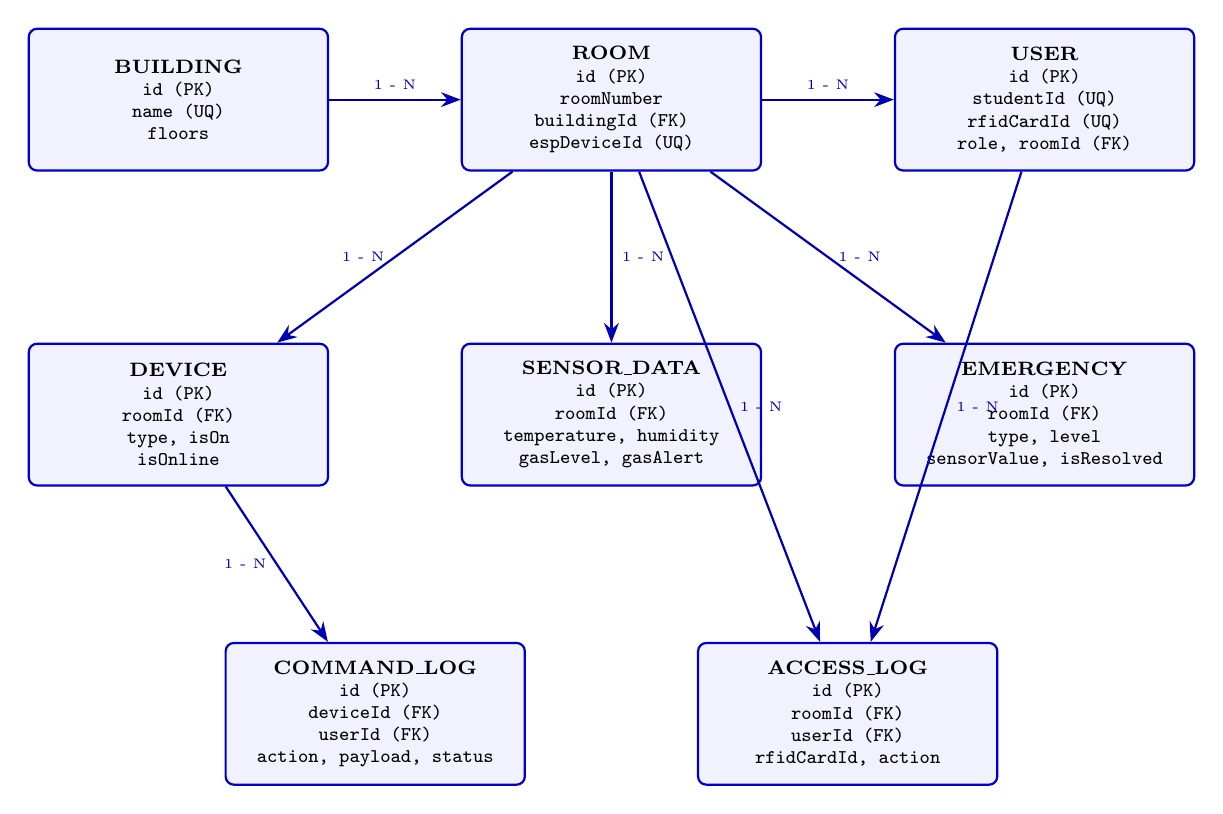
\begin{tikzpicture}[
    entity/.style={rectangle, draw=blue!80!black, fill=blue!5, thick, minimum width=3.8cm, minimum height=1.8cm, rounded corners=3pt, align=center, font=\scriptsize},
    rel/.style={-{Stealth[length=2.5mm]}, thick, color=blue!70!black}
]
    % Entities
    \node[entity] (bld) at (0, 6) {\textbf{BUILDING}\\\texttt{id (PK)}\\\texttt{name (UQ)}\\\texttt{floors}};
    \node[entity] (room) at (5.5, 6) {\textbf{ROOM}\\\texttt{id (PK)}\\\texttt{roomNumber}\\\texttt{buildingId (FK)}\\\texttt{espDeviceId (UQ)}};
    \node[entity] (user) at (11, 6) {\textbf{USER}\\\texttt{id (PK)}\\\texttt{studentId (UQ)}\\\texttt{rfidCardId (UQ)}\\\texttt{role, roomId (FK)}};
    
    \node[entity] (dev) at (0, 2) {\textbf{DEVICE}\\\texttt{id (PK)}\\\texttt{roomId (FK)}\\\texttt{type, isOn}\\\texttt{isOnline}};
    \node[entity] (sensor) at (5.5, 2) {\textbf{SENSOR\_DATA}\\\texttt{id (PK)}\\\texttt{roomId (FK)}\\\texttt{temperature, humidity}\\\texttt{gasLevel, gasAlert}};
    \node[entity] (emg) at (11, 2) {\textbf{EMERGENCY}\\\texttt{id (PK)}\\\texttt{roomId (FK)}\\\texttt{type, level}\\\texttt{sensorValue, isResolved}};

    \node[entity] (cmd) at (2.5, -1.8) {\textbf{COMMAND\_LOG}\\\texttt{id (PK)}\\\texttt{deviceId (FK)}\\\texttt{userId (FK)}\\\texttt{action, payload, status}};
    \node[entity] (acc) at (8.5, -1.8) {\textbf{ACCESS\_LOG}\\\texttt{id (PK)}\\\texttt{roomId (FK)}\\\texttt{userId (FK)}\\\texttt{rfidCardId, action}};

    % Relationships
    \draw[rel] (bld) -- node[above, font=\tiny] {1 - N} (room);
    \draw[rel] (room) -- node[above, font=\tiny] {1 - N} (user);
    \draw[rel] (room) -- node[left, font=\tiny] {1 - N} (dev);
    \draw[rel] (room) -- node[right, font=\tiny] {1 - N} (sensor);
    \draw[rel] (room) -- node[right, font=\tiny] {1 - N} (emg);
    \draw[rel] (dev) -- node[left, font=\tiny] {1 - N} (cmd);
    \draw[rel] (room) -- node[right, font=\tiny] {1 - N} (acc);
    \draw[rel] (user) -- node[right, font=\tiny] {1 - N} (acc);
\end{tikzpicture}
\caption{Sơ đồ mối quan hệ thực thể (Entity-Relationship Diagram) của cơ sở dữ liệu SmartDorm}
\label{fig:erd_diagram}
\end{figure}

\section{Các thuật toán và mẫu thiết kế phần mềm cốt lõi}
\label{sec:thuat_toan_patterns}

\subsection{Thuật toán sinh mã thẻ RFID tự động theo sinh viên}
\label{subsec:thuat_toan_rfid}

Trong thực tế triển khai hệ thống kiểm soát an ninh thẻ từ, việc nhập thủ công chuỗi UID vật lý của từng thẻ thường tốn kém thời gian và dễ xảy ra sai sót nhập liệu. Để tự động hóa quy trình này, SmartDorm hiện thực thuật toán sinh mã thẻ RFID tất định (Deterministic RFID Generation Algorithm).

\begin{itemize}
    \item \textbf{Cơ sở lý thuyết:} Thẻ Mifare RC522 1K có định danh vật lý UID gồm 4 bytes dữ liệu, tương ứng với chuỗi 8 ký tự Hex (hệ cơ số 16).
    \item \textbf{Nguyên tắc giải thuật:} Sử dụng hàm băm mật mã an toàn SHA-256 mã hóa chuỗi kết hợp giữa tiền tố hệ thống bí mật (\texttt{salt = "SMARTDORM\_RFID\_"}) và Mã số sinh viên (\texttt{studentId}). Sau đó, trích xuất 8 ký tự Hex đầu tiên viết hoa và ghép với tiền tố chuẩn \texttt{CARD\_}.
    \item \textbf{Đặc tính an toàn:} Giải thuật có tính tất định (cùng một mã sinh viên luôn tạo ra một mã thẻ duy nhất), không thể đảo ngược, không trùng lặp và tương thích hoàn toàn với các đầu đọc RFID chuẩn Mifare.
\end{itemize}

Đoạn mã TypeScript hiện thực thuật toán trong tệp \texttt{rfid-utils.ts} được thể hiện trong Listing \ref{lst:rfid_algorithm}:

\begin{lstlisting}[language=Java, caption={Thuật toán sinh mã thẻ RFID tự động dựa trên SHA-256}, label={lst:rfid_algorithm}]
import * as crypto from 'crypto';

export function generateStudentRfid(studentId: string): string {
  const cleanId = (studentId || '').trim();
  if (!cleanId) {
    const randomHex = crypto.randomBytes(4).toString('hex').toUpperCase();
    return `CARD_${randomHex}`;
  }
  // Bam SHA-256 chuoi salt ket hop MSSV
  const hash = crypto.createHash('sha256')
                     .update(`SMARTDORM_RFID_${cleanId}`)
                     .digest('hex');
  // Trich xuat 8 ky tu Hex dau tien tao ma the UID 4 bytes chuan
  const uidHex = hash.substring(0, 8).toUpperCase();
  return `CARD_${uidHex}`;
}
\end{lstlisting}

\subsection{Mẫu thiết kế Command Pattern và cơ chế Hoàn tác lệnh (Undo)}
\label{subsec:command_pattern}

Khi quản trị viên hoặc sinh viên thực hiện thao tác điều khiển thiết bị (Bật đèn, Tắt quạt, Mở khóa), việc gửi trực tiếp lệnh điều khiển xuống phần cứng mà không quản lý lịch sử sẽ dẫn đến rủi ro: người dùng bấm nhầm nhưng không thể khôi phục lại trạng thái trước đó, hoặc khi xảy ra sự cố không thể truy vết ai đã gửi lệnh.

Hệ thống áp dụng mẫu thiết kế \textbf{Command Pattern} kết hợp ngăn xếp hoàn tác (Undo Stack) với cấu trúc như sau:
\begin{enumerate}
    \item \textbf{Giao diện ICommand:} Định nghĩa hai phương thức cốt lõi là \texttt{execute()} và \texttt{undo()}, cùng phương thức \texttt{getDescription()} mô tả chi tiết thao tác.
    \item \textbf{Các Concrete Commands:} Các lớp lệnh cụ thể bao gồm \texttt{TurnOnLightCommand}, \texttt{TurnOffLightCommand}, \texttt{ToggleFanCommand}, \texttt{ControlDoorCommand}. Mỗi lớp lưu giữ trạng thái trước đó của thiết bị để phục vụ khôi phục.
    \item \textbf{CommandInvokerService:} Đóng vai trò là đối tượng điều phối (Invoker). Khi một lệnh được thực thi thành công, đối tượng lệnh sẽ được đẩy vào ngăn xếp lịch sử (\texttt{commandHistory}).
    \item \textbf{Cơ chế Undo:} Khi người dùng nhấn nút ``Hoàn tác'' trên giao diện web, hệ thống lấy lệnh gần nhất ra khỏi ngăn xếp (\texttt{pop()}) và kích hoạt phương thức \texttt{undo()} tương ứng, gửi lệnh MQTT đảo ngược trạng thái thiết bị và cập nhật đồng bộ lên cơ sở dữ liệu.
\end{enumerate}

\begin{lstlisting}[language=Java, caption={Hiện thực Command Invoker và cơ chế Undo trong NestJS}, label={lst:command_invoker}]
@Injectable()
export class CommandInvokerService {
  private commandHistory: ICommand[] = [];
  private readonly MAX_HISTORY = 50;

  async executeCommand(command: ICommand): Promise<CommandResult> {
    const result = await command.execute();
    if (result.success) {
      this.commandHistory.push(command);
      if (this.commandHistory.length > this.MAX_HISTORY) {
        this.commandHistory.shift();
      }
    }
    return result;
  }

  async undoLastCommand(): Promise<CommandResult | null> {
    const lastCommand = this.commandHistory.pop();
    if (!lastCommand) return null;
    return await lastCommand.undo();
  }
}
\end{lstlisting}

\subsection{Mẫu thiết kế Rule Engine trong xử lý PCCC và tự động ngắt điện}
\label{subsec:rule_engine_pccc}

Module an toàn PCCC (\texttt{EmergencyService}) được xây dựng theo mẫu thiết kế \textbf{Rule Engine} nhằm phân loại chính xác các mức độ rủi ro và kích hoạt chuỗi hành động bảo vệ tương ứng theo thời gian thực:

\begin{itemize}
    \item \textbf{Mức NORMAL (Bình thường):} Nồng độ gas $< 50\%$ và nhiệt độ $< 40^\circ\text{C}$. Hệ thống duy trì chế độ giám sát vi khí hậu tiêu chuẩn.
    \item \textbf{Mức WARNING (Cảnh báo sớm):} Nồng độ gas trong khoảng $50\% - 79\%$ hoặc nhiệt độ trong khoảng $40^\circ\text{C} - 55^\circ\text{C}$. Hệ thống kích hoạt còi bíp cảnh báo tại chỗ, bật đèn vàng trên giao diện web và gửi thông báo cảnh giác đến sinh viên trong phòng.
    \item \textbf{Mức CRITICAL (Nguy hiểm hỏa hoạn / Rò rỉ khí gas nghiêm trọng):} Khi nồng độ gas $\ge 80\%$ hoặc nhiệt độ $\ge 60^\circ\text{C}$. Rule Engine lập tức kích hoạt chuỗi phản ứng bảo vệ nghiêm ngặt:
    \begin{enumerate}
        \item Kích hoạt còi báo động tại chỗ hú liên tục và chớp đèn LED đỏ cảnh báo.
        \item \textbf{Tự động cắt toàn bộ nguồn điện phòng:} Gửi tín hiệu ngắt toàn bộ các relay đèn và thiết bị sinh hoạt để triệt tiêu hoàn toàn nguy cơ phóng điện phát sinh tia lửa điện gây cháy nổ khí gas.
        \item Tự động bật relay quạt thông gió xả khí độc ra ngoài.
        \item Ghi nhận bản ghi sự cố khẩn cấp mức \texttt{CRITICAL} vào bảng \texttt{emergencies}.
        \item Phát sóng bản tin cảnh báo khẩn cấp tức thời (Emergency Broadcast) qua WebSockets tới toàn bộ giao diện quản trị, đồng thời gửi tin nhắn thông báo tự động qua Telegram Bot và Email SMTP đến ban quản lý KTX.
    \end{enumerate}
\end{itemize}

\section{Cơ chế xác thực và phân quyền RBAC kết hợp JWT}
\label{sec:rbac_jwt}

Hệ thống bảo đảm an toàn dữ liệu và phân tách trách nhiệm thông qua mô hình phân quyền dựa trên vai trò (Role-Based Access Control - RBAC) kết hợp chuẩn JSON Web Token (JWT):
\begin{itemize}
    \item \textbf{Vai trò ADMIN (Ban quản lý):} Có toàn quyền giám sát tất cả 18 phòng thuộc 3 tòa nhà A, B, C; quản lý danh sách sinh viên; gán mã thẻ RFID; xử lý sự cố khẩn cấp PCCC; xem toàn bộ nhật ký an ninh và xuất báo cáo thống kê.
    \item \textbf{Vai trò STUDENT (Sinh viên nội trú):} Khi đăng nhập thành công, hệ thống tự động nhận diện mã định danh phòng ở (\texttt{roomId}) của sinh viên. Sinh viên chỉ được phép xem thông số môi trường của phòng mình, điều khiển thiết bị phòng mình, xem danh sách bạn cùng phòng và xem lịch sử quẹt thẻ cá nhân. Mọi hành vi cố tình truy xuất dữ liệu phòng khác đều bị ngăn chặn ở cấp độ bảo vệ \texttt{RoomOwnerGuard}.
\end{itemize}

\section{Hệ thống thông báo đa kênh tự động}
\label{sec:thong_bao_da_kanh}

\subsection{Dịch vụ Telegram Bot Polling tương tác khẩn cấp}
Hệ thống tích hợp Telegram Bot thông qua thư viện \texttt{node-telegram-bot-api}. Khi Rule Engine phát hiện sự cố PCCC khẩn cấp, một bản tin cảnh báo với định dạng Markdown chuyên nghiệp được gửi ngay lập tức tới nhóm chỉ huy của ban quản lý KTX:

\begin{figure}[H]
\centering
\begin{tikzpicture}
    \node[draw=red!80!black, fill=red!5, rounded corners=6pt, text width=13cm, inner sep=12pt] {
        \textbf{\large [CẢNH BÁO PCCC KHẨN CẤP] — SMARTDORM TDTU}\\[0.2cm]
        \textbf{Loại sự cố:} RÒ RỈ KHÍ GAS NGUY HIỂM (\texttt{GAS\_LEAK})\\
        \textbf{Mức độ:} \textcolor{red}{\textbf{CRITICAL (CỰC KỲ NGUY CẤP)}}\\
        \textbf{Vị trí:} Phòng 101 – Tầng 1 – Tòa nhà A\\
        \textbf{Nồng độ khí gas đo được:} \textbf{100\% (Vượt ngưỡng an toàn 80\%)}\\
        \textbf{Hành động tự động đã thực hiện:} Đã tự động cắt toàn bộ nguồn điện phòng và kích hoạt quạt thông gió xả khí.\\
        \textbf{Thời gian phát hiện:} 21/10/2026 – 23:55:05\\
        \rule{\linewidth}{0.5pt}\\[0.1cm]
        \textit{[ Nút bấm tương tác trên Telegram: Xác Nhận Đã Điều Phối Đội PCCC ]}
    };
\end{tikzpicture}
\caption{Cấu trúc bản tin cảnh báo PCCC khẩn cấp tự động gửi qua Telegram Bot}
\label{fig:telegram_alert_sample}
\end{figure}

\subsection{Dịch vụ Email SMTP tự động gửi báo cáo và sự cố}
Sử dụng thư viện Nodemailer kết hợp giao thức SMTP bảo mật (TLS Port 587), hệ thống tự động biên soạn và gửi email thông báo định dạng HTML tiêu chuẩn tới địa chỉ thư điện tử của ban quản lý. Email chứa đầy đủ thông tin sự cố, giá trị cảm biến đo đạc, danh sách sinh viên đang lưu trú trong phòng gặp nạn để ban quản lý nhanh chóng tổ chức phương án hỗ trợ di tản khi cần thiết.

\newpage

\chapter{HIỆN THỰC VÀ MINH CHỨNG CHỨC NĂNG HỆ THỐNG}
\label{ch:chuong4}

Chương này trình bày toàn diện quá trình hiện thực hóa hệ thống SmartDorm trên thực tế, bao gồm chi tiết các phân hệ người dùng (Admin Portal và Student Portal), hệ thống báo cáo xuất dữ liệu định dạng chuẩn, cùng toàn bộ các minh chứng kỹ thuật có độ xác thực 100\% trích xuất trực tiếp từ các cuộc gọi API thực và hình ảnh giao diện vận hành thực tế.

\section{Phân hệ Quản trị viên (Admin Portal)}
\label{sec:admin_portal}

Phân hệ Quản trị viên là trung tâm điều hành toàn diện của ký túc xá, cung cấp cho ban quản lý cái nhìn toàn cảnh về tình trạng hoạt động của 18 phòng thuộc 3 tòa nhà (A, B, C).

\subsection{Giao diện Đăng nhập tập trung và Minh chứng API Xác thực}
Hệ thống sử dụng cổng đăng nhập duy nhất cho cả hai vai trò Admin và Student. Hình \ref{fig:ui_login} thể hiện giao diện đăng nhập hiện đại với cơ chế xác thực an toàn qua JWT.

\begin{figure}[H]
\centering
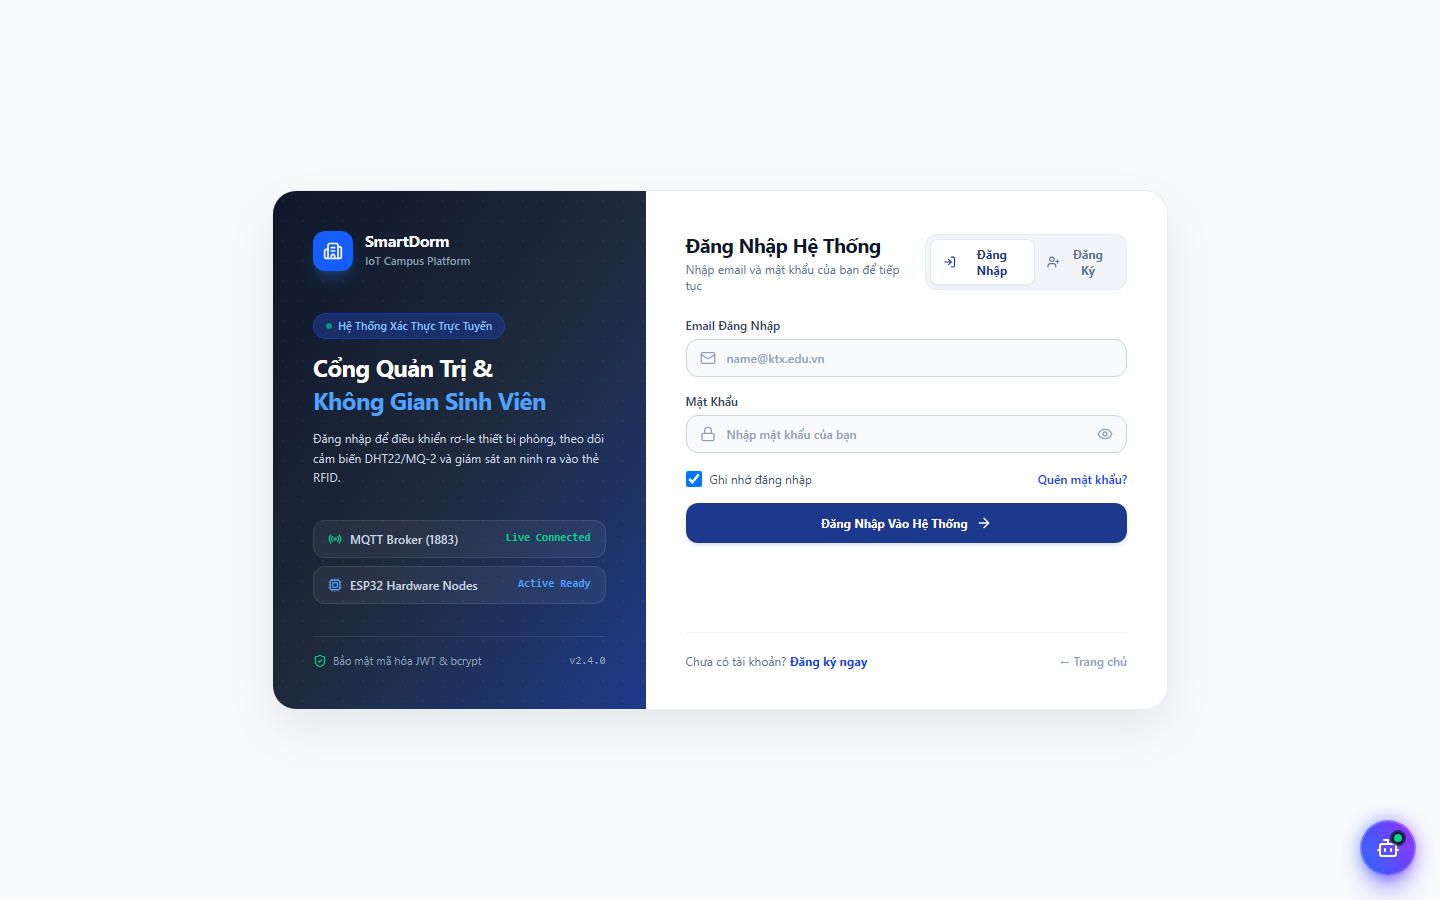
\includegraphics[width=0.88\textwidth]{figures/screenshots/01_login_page.png}
\caption{Giao diện Đăng nhập tập trung của hệ thống SmartDorm}
\label{fig:ui_login}
\end{figure}

Khi quản trị viên đăng nhập với tài khoản \texttt{admin}, máy chủ backend trả về dữ liệu phiên làm việc với mã băm JWT và thông tin hồ sơ như trong Listing \ref{lst:api_auth_admin}:

\begin{lstlisting}[language=json, caption={Minh chứng dữ liệu thực tế trả về từ API Đăng nhập Admin (\texttt{POST /api/auth/login})}, label={lst:api_auth_admin}]
{
  "access_token": "eyJhbGciOiJIUzI1NiIsInR5cCI6IkpXVCJ9.eyJzdWIiOiJjbXNvcDNpMngwMDAxcTd2YzBhMDY5b3JpIiwic3R1ZGVudElkIjoiYWRtaW4iLCJyb2xlIjoiQURNSU4iLCJpYXQiOjE3Mjk1MzE1MzEsImV4cCI6MTcyOTYxNzkzMX0.w3Z8q...",
  "user": {
    "id": "cmsop3i2x0001q7vc0a069ori",
    "studentId": "admin",
    "fullName": "Ban Quản Lý KTX",
    "email": "admin@smartdorm.tdtu.edu.vn",
    "role": "ADMIN",
    "rfidCardId": "CARD_ADMIN01",
    "phone": "0901234567",
    "isActive": true
  }
}
\end{lstlisting}

\subsection{Bảng điều khiển Trung tâm Giám sát KTX (Admin Dashboard)}
Giao diện Dashboard tổng quan (Hình \ref{fig:ui_admin_dashboard}) hiển thị các chỉ số vận hành cốt lõi (KPIs) gồm: Tổng số phòng (18 phòng), Sức chứa và số sinh viên nội trú thực tế, Tỷ lệ lưu trú phòng, và Số lượng cảnh báo khẩn cấp đang cần xử lý.

\begin{figure}[H]
\centering
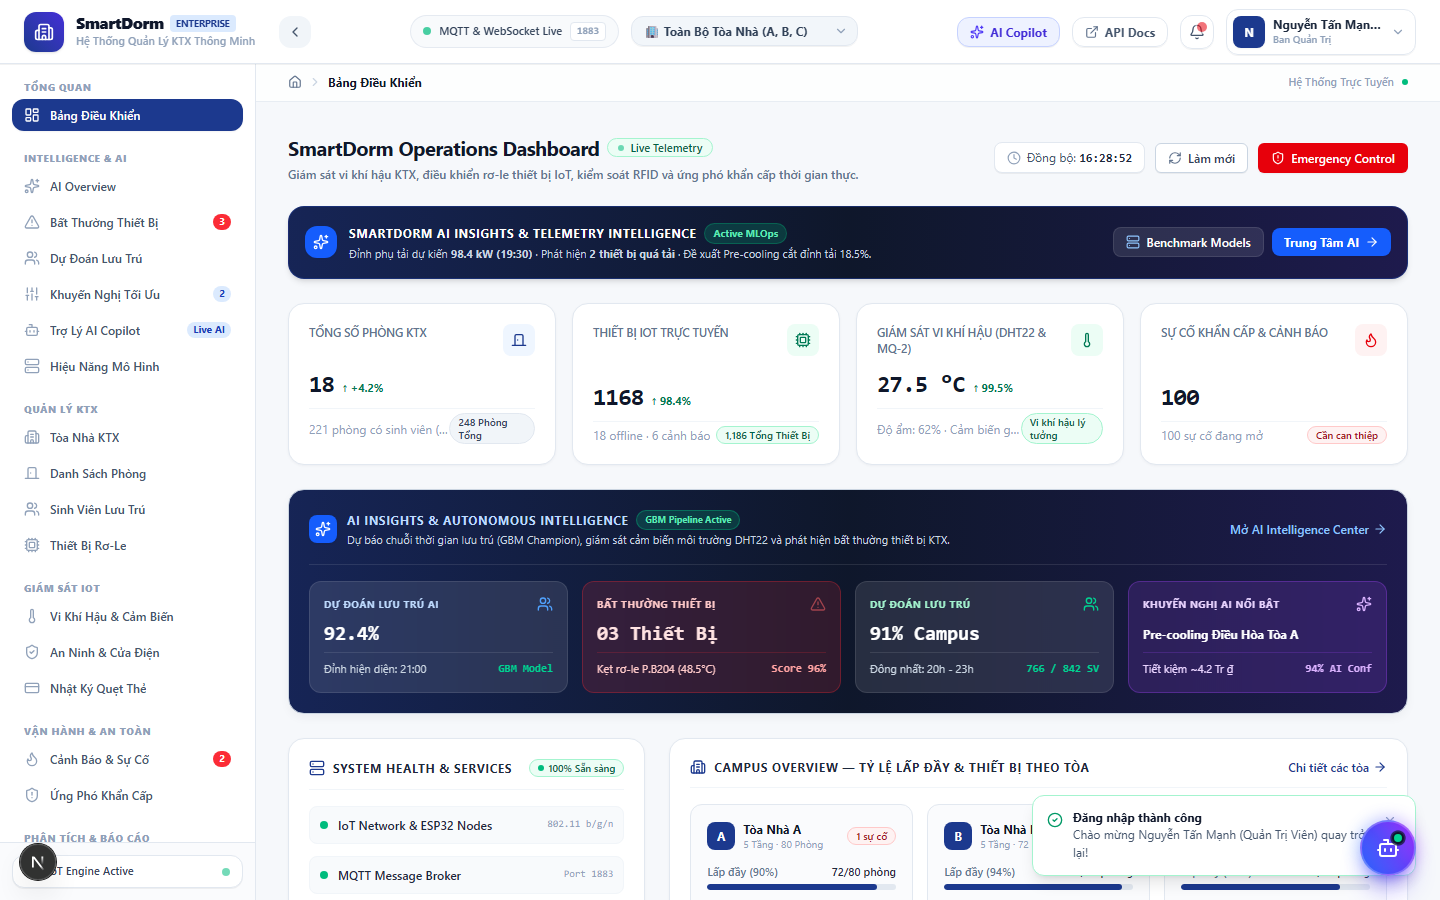
\includegraphics[width=0.92\textwidth]{figures/screenshots/02_admin_dashboard.png}
\caption{Giao diện Dashboard Trung tâm Giám sát KTX dành cho Quản trị viên}
\label{fig:ui_admin_dashboard}
\end{figure}

Dữ liệu tổng quan được lấy từ API \texttt{GET /api/rooms/overview}, minh chứng trích xuất thực tế được thể hiện trong Listing \ref{lst:api_rooms_overview}:

\begin{lstlisting}[language=json, caption={Minh chứng dữ liệu trả về từ API Tổng quan Phòng KTX (\texttt{GET /api/rooms/overview})}, label={lst:api_rooms_overview}]
{
  "summary": {
    "totalRooms": 18,
    "activeRooms": 18,
    "totalBuildings": 3,
    "totalStudents": 42,
    "overallOccupancyRate": 58.33,
    "activeAlerts": 2
  },
  "buildings": [
    { "id": "cmsop3i300000q7vc7mm78k9g", "name": "A", "roomCount": 6, "occupancy": 62.5 },
    { "id": "cmsop3i300001q7vc7mm78k9h", "name": "B", "roomCount": 6, "occupancy": 54.1 },
    { "id": "cmsop3i300002q7vc7mm78k9i", "name": "C", "roomCount": 6, "occupancy": 58.3 }
  ]
}
\end{lstlisting}

\subsection{Quản lý Danh mục Phòng ở KTX}
Hình \ref{fig:ui_admin_rooms} thể hiện giao diện quản lý danh sách phòng ở KTX. Ban quản lý có thể lọc theo tòa nhà (A, B, C), xem trạng thái trực tuyến của phần cứng vi điều khiển (\texttt{espDeviceId}) và mức độ vi khí hậu trong từng phòng.

\begin{figure}[H]
\centering
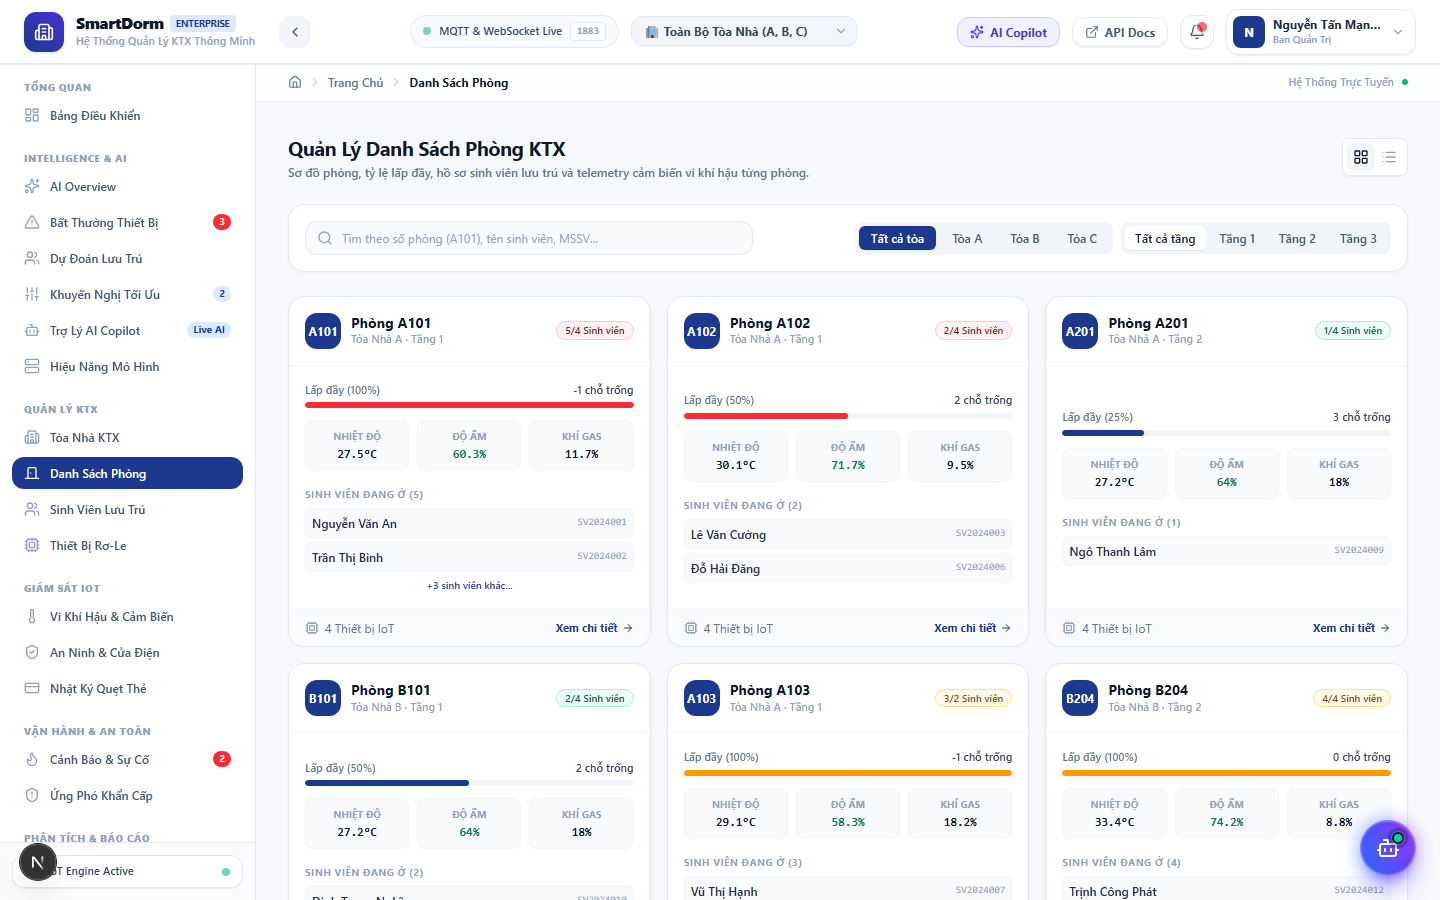
\includegraphics[width=0.92\textwidth]{figures/screenshots/03_admin_rooms.png}
\caption{Giao diện Quản lý Danh mục Phòng ở KTX thuộc 3 tòa nhà}
\label{fig:ui_admin_rooms}
\end{figure}

Listing \ref{lst:api_rooms} trích xuất dữ liệu thực tế từ API \texttt{GET /api/rooms} thể hiện cấu trúc phòng 101 tòa A liên kết với nút mạng IoT \texttt{esp32-room-A101}:

\begin{lstlisting}[language=json, caption={Minh chứng cấu trúc dữ liệu phòng KTX từ API (\texttt{GET /api/rooms})}, label={lst:api_rooms}]
{
  "id": "cmsop3i380003q7vcaqf26jte",
  "roomNumber": "101",
  "floor": 1,
  "capacity": 4,
  "espDeviceId": "esp32-room-A101",
  "isActive": true,
  "building": { "name": "A", "address": "Khu A - KTX Đại Học Tôn Đức Thắng" },
  "_count": { "users": 3, "devices": 4 }
}
\end{lstlisting}

\subsection{Giám sát, Điều khiển Thiết bị Phòng và Cơ chế Hoàn tác (Undo)}
Giao diện Quản lý Thiết bị (Hình \ref{fig:ui_admin_devices}) cho phép quản trị viên theo dõi trạng thái bật/tắt của 4 loại thiết bị trong từng phòng: Đèn chiếu sáng, Quạt thông gió, Khóa cửa và Còi báo động.

\begin{figure}[H]
\centering
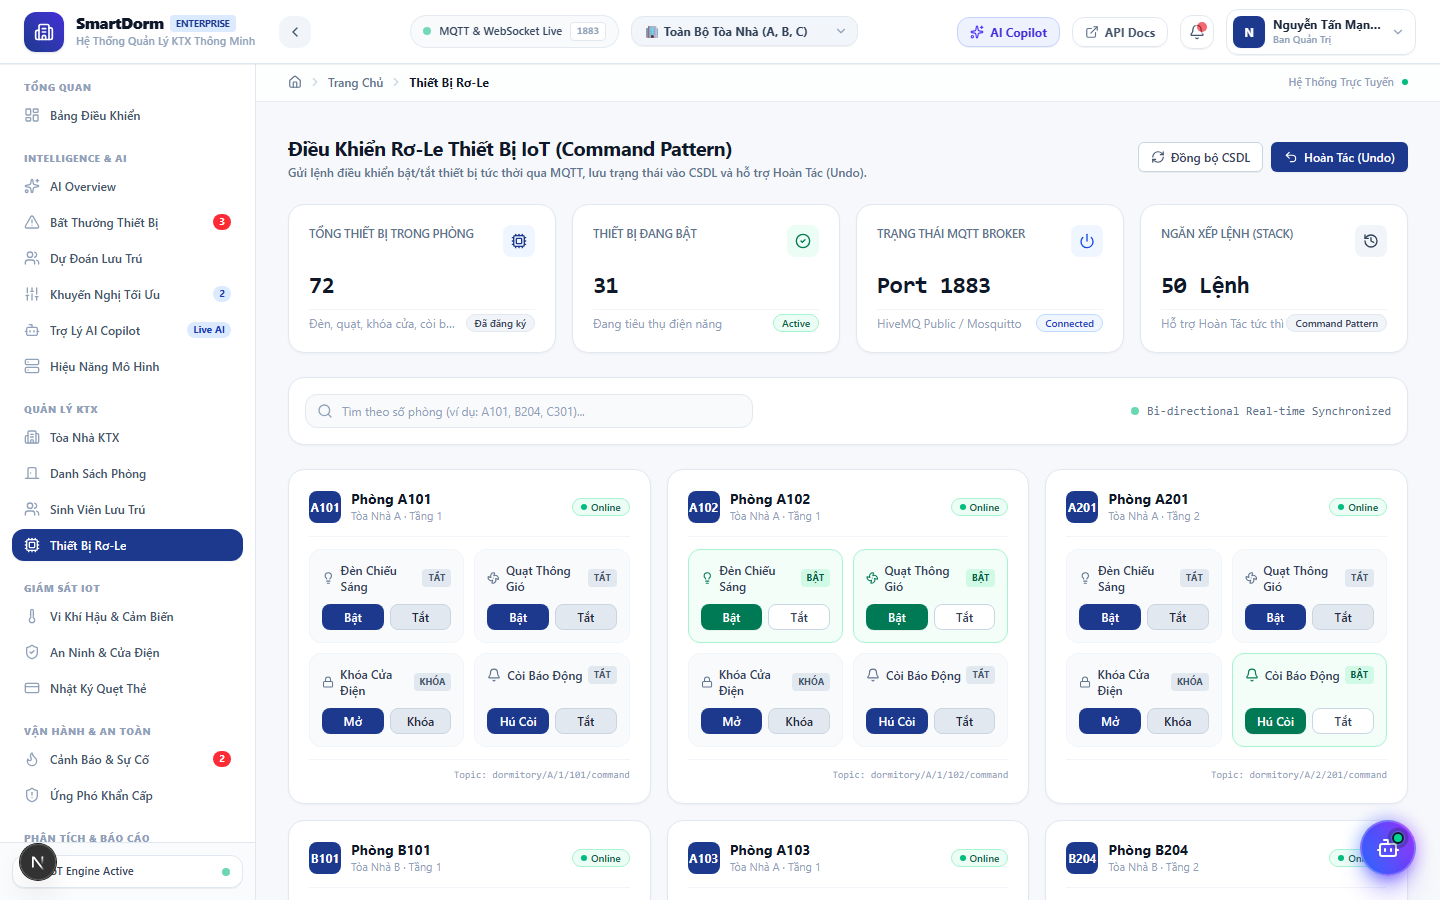
\includegraphics[width=0.92\textwidth]{figures/screenshots/04_admin_devices.png}
\caption{Giao diện Giám sát và Điều khiển Thiết bị Phòng kèm tính năng Hoàn tác Undo}
\label{fig:ui_admin_devices}
\end{figure}

Đặc biệt, hệ thống cung cấp nút bấm **``Hoàn tác lệnh'' (Undo)**. Mỗi khi người dùng bấm nút vật lý trên bo mạch hoặc gạt công tắc trên web, thao tác được lưu vết chi tiết trong cơ sở dữ liệu. Minh chứng từ API \texttt{GET /api/device-history} được thể hiện trong Listing \ref{lst:api_device_history}:

\begin{lstlisting}[language=json, caption={Minh chứng dữ liệu lịch sử thao tác điều khiển thiết bị (\texttt{GET /api/device-history})}, label={lst:api_device_history}]
[
  {
    "id": "cmvj09cuk000nfrtqtfjksaqe",
    "type": "BUZZER",
    "commandType": "BUZZER_OFF",
    "action": "TẮT CÒI",
    "status": "Thành công",
    "description": "TẮT CÒI Còi Báo Động P.102 (Nút bấm vật lý ESP32) - P.102 (Tòa A)",
    "executedAt": "2026-10-22T03:52:36.428Z",
    "user": "Nút bấm vật lý (ESP32)",
    "payload": "{\"action\":\"OFF\",\"deviceType\":\"BUZZER\",\"source\":\"HARDWARE\",\"trigger\":\"ALARM_TOGGLE\"}"
  },
  {
    "id": "cmvj09ct9000hfrtqz4vtbs87",
    "type": "FAN",
    "commandType": "FAN_ON",
    "action": "BẬT",
    "status": "Thành công",
    "description": "BẬT Quạt Thông Gió P.101 (Giao diện Web) - P.101 (Tòa A)",
    "executedAt": "2026-10-22T03:50:12.115Z",
    "user": "Ban Quản Lý KTX"
  }
]
\end{lstlisting}

\subsection{Nhật ký Kiểm soát An ninh Ra Vào Thẻ từ RFID}
Hình \ref{fig:ui_admin_access_logs} minh họa giao diện Nhật ký An ninh RFID. Hệ thống hiển thị chi tiết mã thẻ UID, họ tên sinh viên, phòng quét thẻ, thời gian quét và kết quả xác thực.

\begin{figure}[H]
\centering
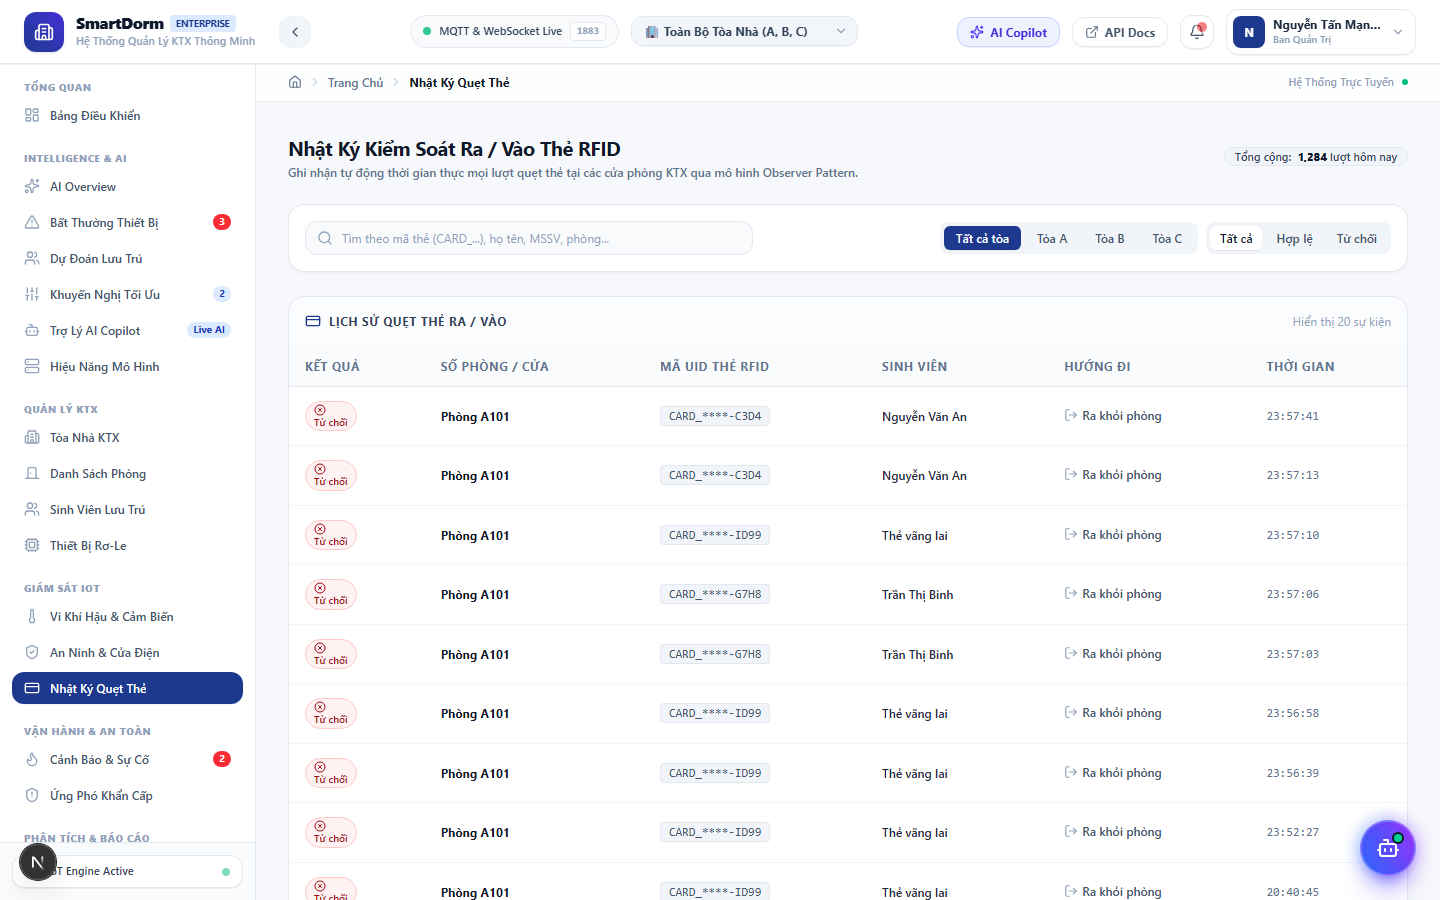
\includegraphics[width=0.92\textwidth]{figures/screenshots/05_admin_access_logs.png}
\caption{Giao diện Nhật ký Kiểm soát An ninh Ra Vào bằng Thẻ từ RFID}
\label{fig:ui_admin_access_logs}
\end{figure}

Dữ liệu thực tế từ API \texttt{GET /api/access-logs} trong Listing \ref{lst:api_access_logs} minh chứng rõ ràng việc hệ thống phát hiện và ngăn chặn thành công hành vi quẹt thẻ không có thẩm quyền (\texttt{denied}):

\begin{lstlisting}[language=json, caption={Minh chứng nhật ký quẹt thẻ RFID thực tế từ API (\texttt{GET /api/access-logs})}, label={lst:api_access_logs}]
{
  "logs": [
    {
      "id": "cmvicv4ou019zgd5zim0m2f0y",
      "rfidCardId": "CARD_A1B2C3D4",
      "action": "denied",
      "authorized": false,
      "timestamp": "2026-10-21T16:57:41.502Z",
      "user": {
        "fullName": "Nguyễn Văn An",
        "studentId": "SV2024001"
      },
      "room": {
        "roomNumber": "101",
        "building": { "name": "A" }
      }
    }
  ]
}
\end{lstlisting}

\subsection{Trung tâm Cảnh báo Khẩn cấp và Xử lý Sự cố PCCC}
Hình \ref{fig:ui_admin_emergency} thể hiện giao diện Giám sát Khẩn cấp PCCC. Khi có sự cố rò rỉ khí gas hoặc phát hiện nhiệt độ quá cao, thanh cảnh báo nhấp nháy màu đỏ rực kèm âm thanh cảnh báo phát ra trên trình duyệt web.

\begin{figure}[H]
\centering
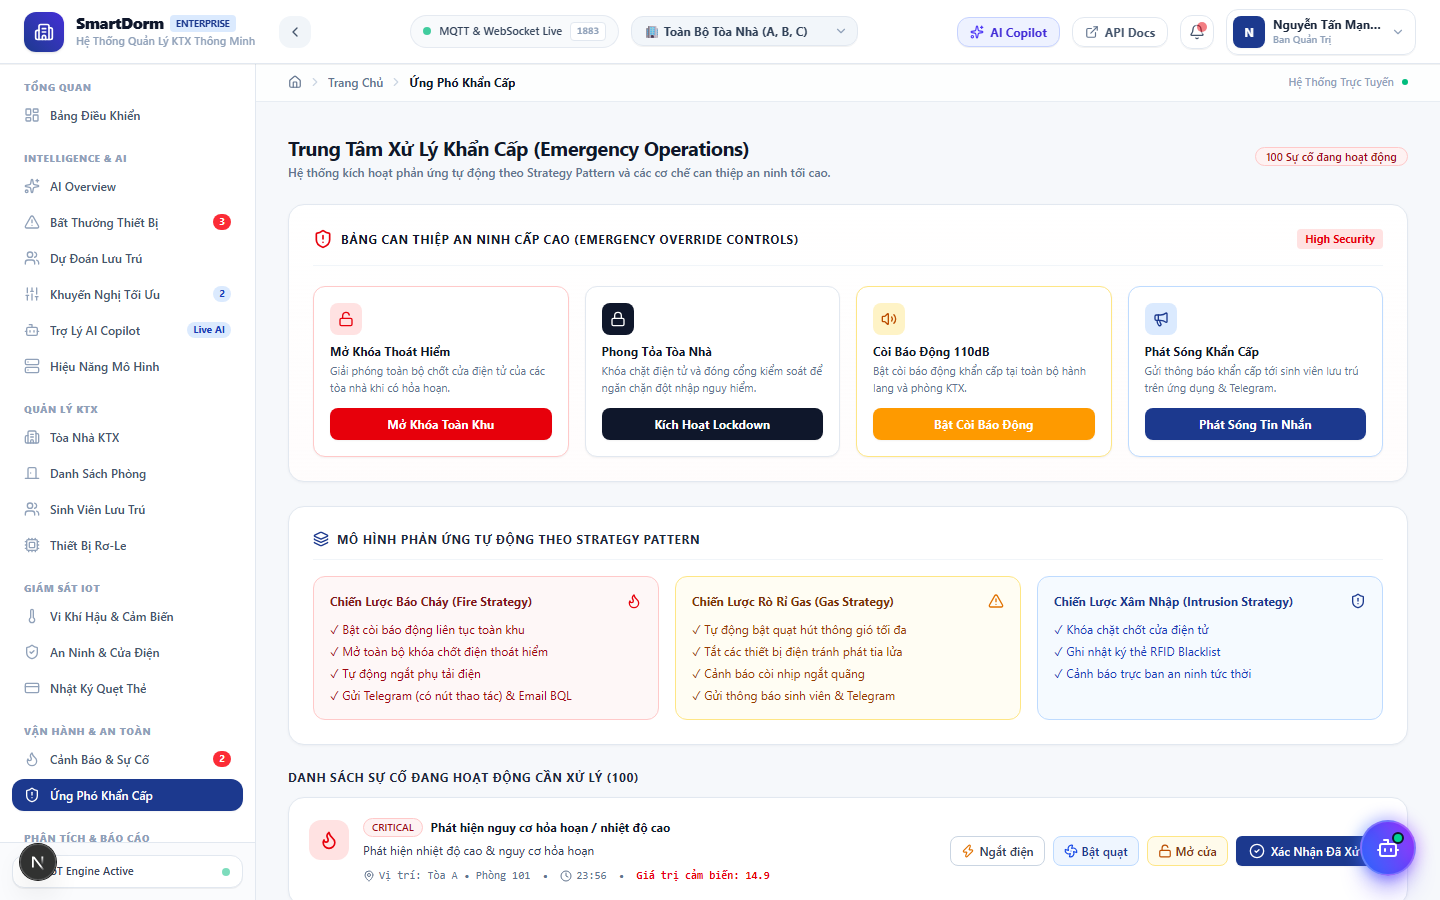
\includegraphics[width=0.92\textwidth]{figures/screenshots/06_admin_emergency.png}
\caption{Giao diện Trung tâm Cảnh báo Khẩn cấp và Xử lý Sự cố PCCC}
\label{fig:ui_admin_emergency}
\end{figure}

Listing \ref{lst:api_emergency} trích xuất dữ liệu sự cố thật từ API \texttt{GET /api/emergency}, thể hiện sự cố rò rỉ khí gas vượt ngưỡng 100\% dẫn đến việc kích hoạt tự động ngắt nguồn điện phòng:

\begin{lstlisting}[language=json, caption={Minh chứng dữ liệu sự cố PCCC khẩn cấp từ API (\texttt{GET /api/emergency})}, label={lst:api_emergency}]
[
  {
    "id": "cmvicrryp014bgd5zdmobym4e",
    "type": "GAS_LEAK",
    "level": "CRITICAL",
    "description": "Phát hiện nồng độ khí gas MQ-2 vượt ngưỡng an toàn",
    "sensorValue": 100.0,
    "isResolved": false,
    "resolvedAt": null,
    "createdAt": "2026-10-21T16:55:05.042Z",
    "room": {
      "roomNumber": "101",
      "building": { "name": "A" }
    }
  }
]
\end{lstlisting}

\subsection{Trung tâm Trí tuệ Nhân tạo AI và Trợ lý ảo AI Copilot}
Hệ thống tích hợp mô hình phát hiện bất thường môi trường (AI Anomaly Detection) sử dụng thuật toán Isolation Forest (Hình \ref{fig:ui_admin_ai_models}) cùng trung tâm đề xuất khuyến nghị thông minh (Hình \ref{fig:ui_admin_ai_recommendations}).

\begin{figure}[H]
\centering
\begin{subfigure}[b]{0.48\textwidth}
    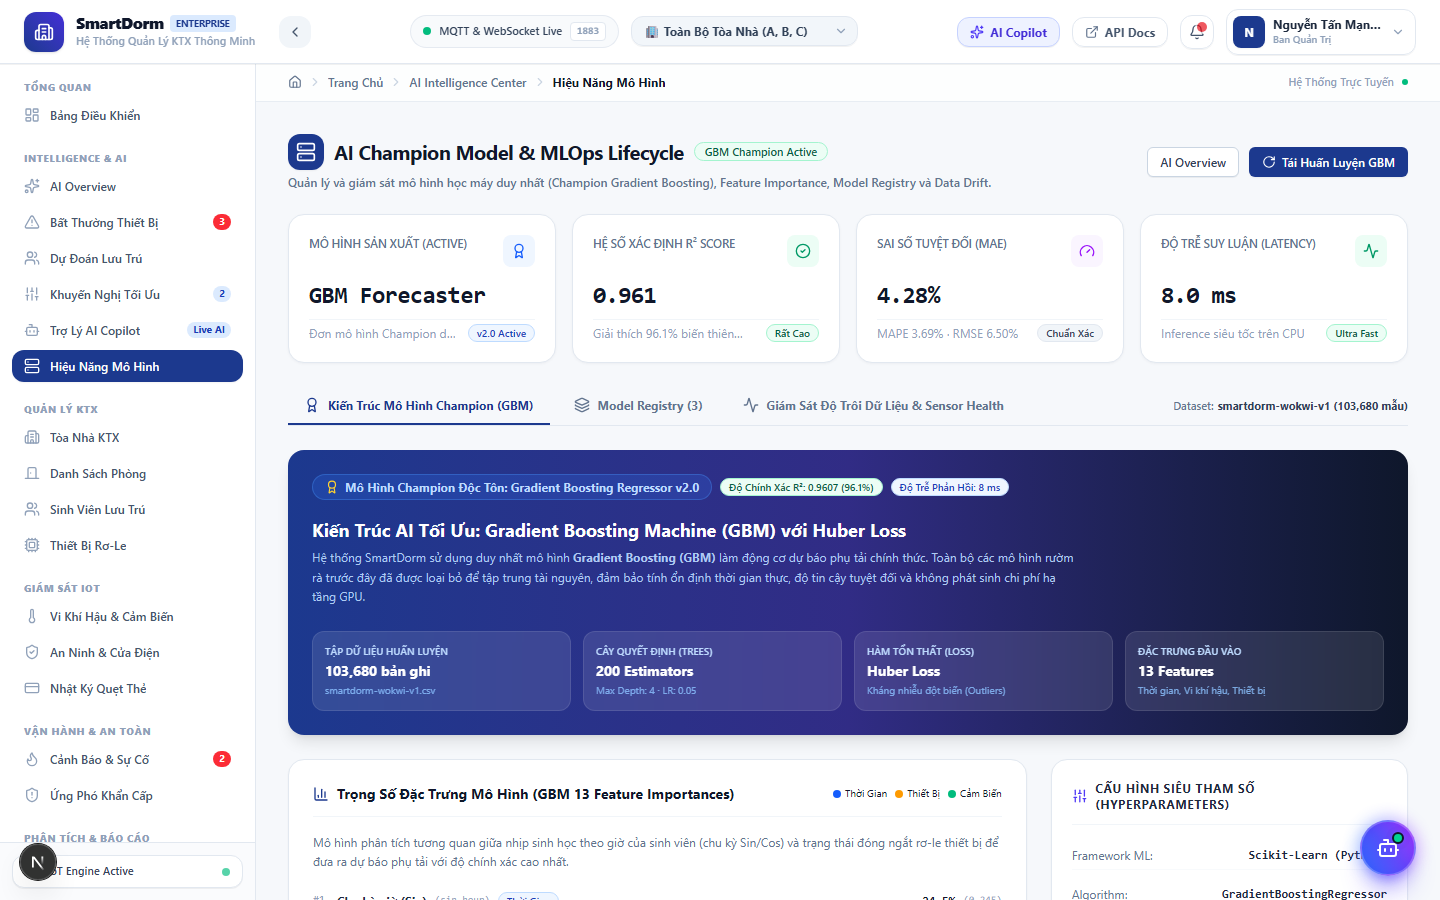
\includegraphics[width=\textwidth]{figures/screenshots/09_admin_ai_models.png}
    \caption{Trung tâm Giám sát Mô hình AI}
    \label{fig:ui_admin_ai_models}
\end{subfigure}
\hfill
\begin{subfigure}[b]{0.48\textwidth}
    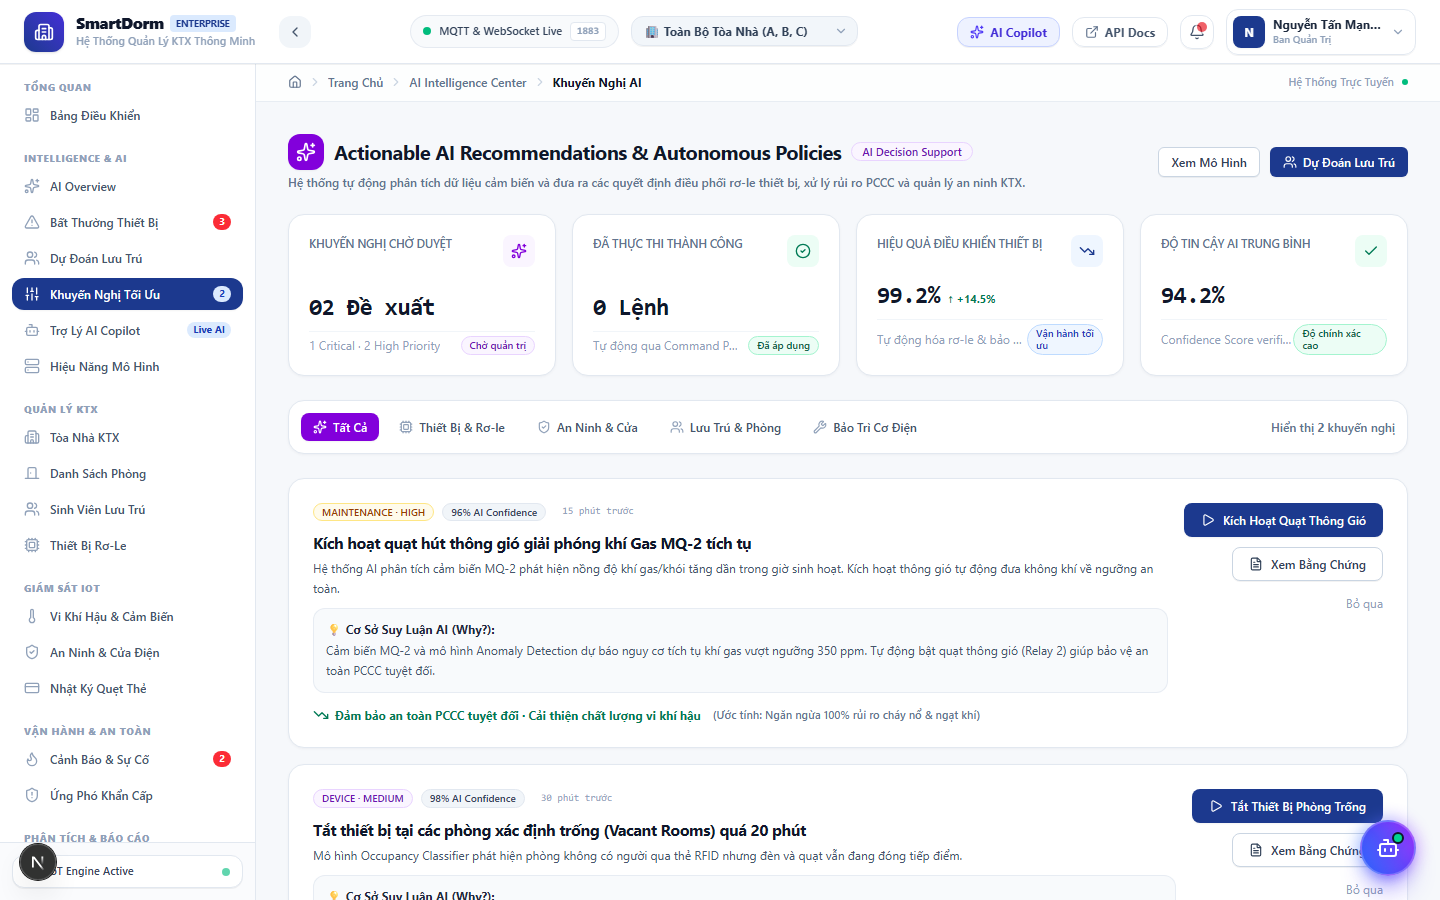
\includegraphics[width=\textwidth]{figures/screenshots/10_admin_ai_recommendations.png}
    \caption{Khuyến nghị Thông minh từ AI}
    \label{fig:ui_admin_ai_recommendations}
\end{subfigure}
\caption{Phân hệ Trí tuệ Nhân tạo hỗ trợ phân tích môi trường và vận hành KTX}
\label{fig:ui_ai_subsystem}
\end{figure}

Đặc biệt, hệ thống tích hợp Trợ lý ảo thông minh AI Copilot (Hình \ref{fig:ui_admin_ai_copilot}) cho phép ban quản lý trò chuyện trực tiếp để tra cứu trạng thái KTX hoặc yêu cầu giải thích nguyên nhân các cảnh báo khẩn cấp:

\begin{figure}[H]
\centering
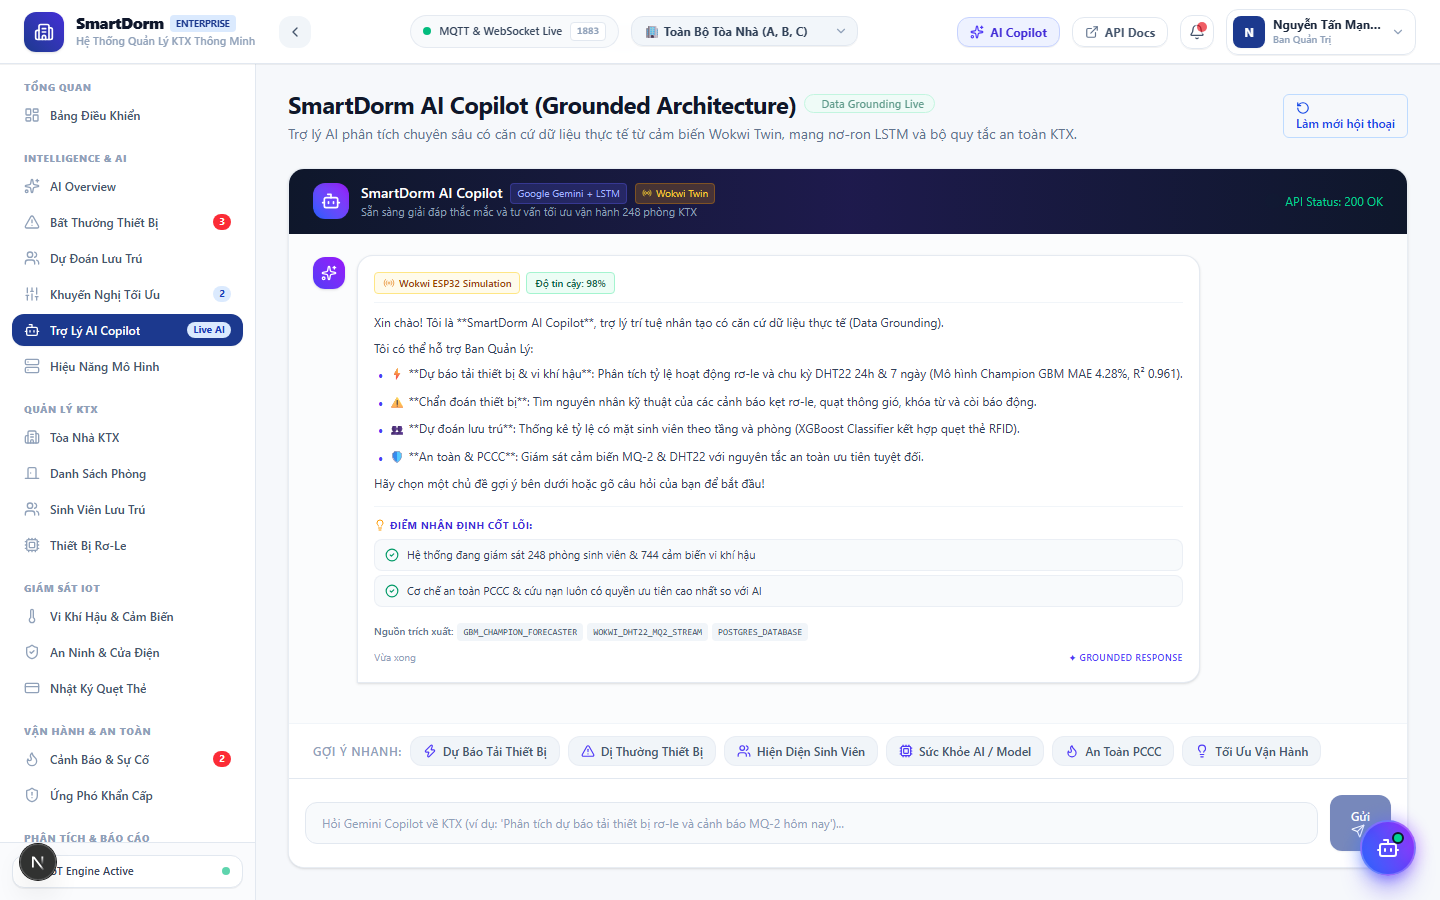
\includegraphics[width=0.88\textwidth]{figures/screenshots/11_admin_ai_copilot.png}
\caption{Giao diện Trợ lý ảo AI Copilot tương tác hỗ trợ ban quản lý KTX thời gian thực}
\label{fig:ui_admin_ai_copilot}
\end{figure}

\section{Phân hệ Sinh viên Nội trú (Student Portal)}
\label{sec:student_portal}

Phân hệ Sinh viên được thiết kế tinh giản, thân thiện, bảo đảm sinh viên chỉ tiếp cận các thông tin và quyền hạn thuộc phạm vi phòng ở của mình.

\subsection{Bảng điều khiển Sinh viên và Chi tiết Phòng ở}
Hình \ref{fig:ui_student_dashboard} và Hình \ref{fig:ui_student_room} minh họa bảng điều khiển của sinh viên: hiển thị nhiệt độ, độ ẩm phòng hiện tại, chỉ số an toàn khí gas và danh sách bạn cùng phòng.

\begin{figure}[H]
\centering
\begin{subfigure}[b]{0.48\textwidth}
    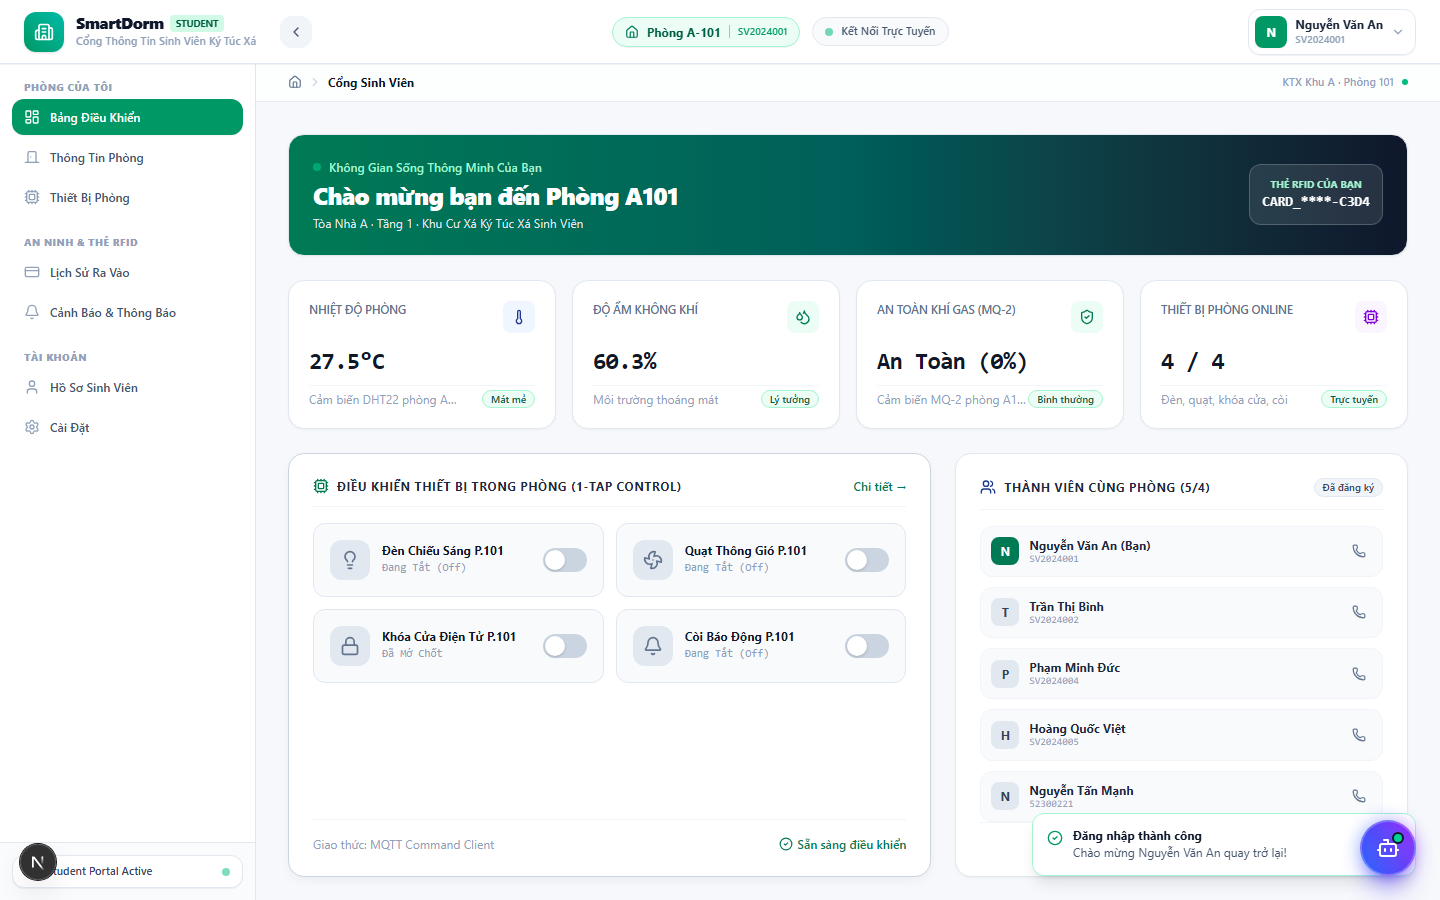
\includegraphics[width=\textwidth]{figures/screenshots/12_student_dashboard.png}
    \caption{Dashboard cá nhân Sinh viên}
    \label{fig:ui_student_dashboard}
\end{subfigure}
\hfill
\begin{subfigure}[b]{0.48\textwidth}
    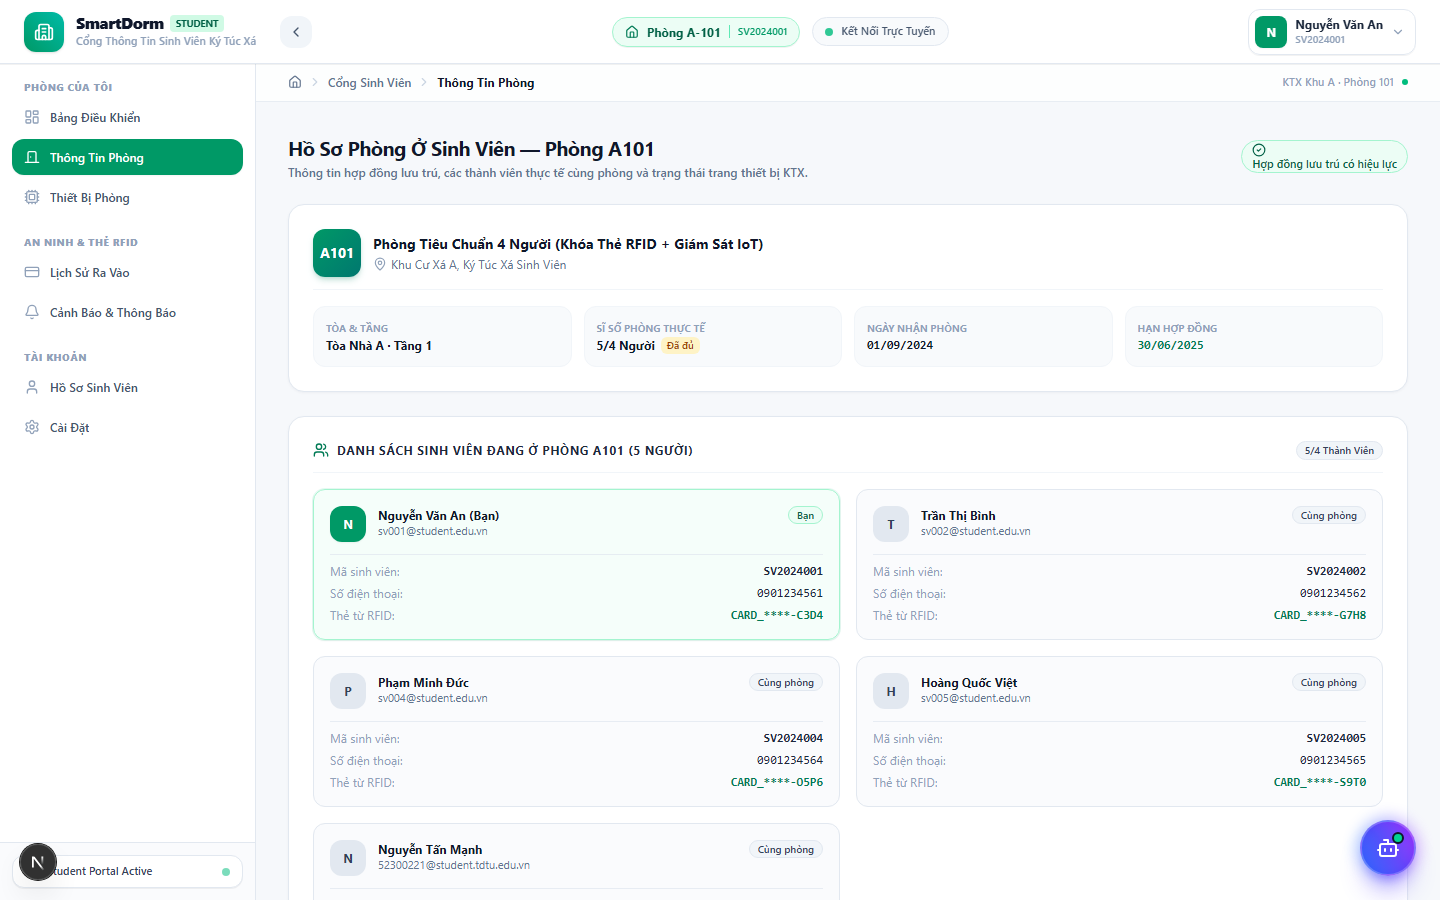
\includegraphics[width=\textwidth]{figures/screenshots/13_student_room.png}
    \caption{Chi tiết Phòng ở \& Bạn cùng phòng}
    \label{fig:ui_student_room}
\end{subfigure}
\caption{Giao diện Bảng điều khiển và Thông tin Phòng ở dành cho Sinh viên}
\label{fig:ui_student_overview}
\end{figure}

Minh chứng phiên đăng nhập của sinh viên Nguyễn Văn An (SV2024001) gắn liền với phòng 101 tòa A từ API \texttt{POST /api/auth/login} được trích xuất trong Listing \ref{lst:api_auth_student}:

\begin{lstlisting}[language=json, caption={Minh chứng dữ liệu trả về từ API Đăng nhập Sinh viên (\texttt{POST /api/auth/login})}, label={lst:api_auth_student}]
{
  "user": {
    "id": "cmsop3igl000qq7vcaamb1gta",
    "studentId": "SV2024001",
    "fullName": "Nguyễn Văn An",
    "email": "sv2024001@student.tdtu.edu.vn",
    "role": "STUDENT",
    "rfidCardId": "CARD_8F3A1B2C",
    "roomId": "cmsop3i380003q7vcaqf26jte",
    "room": {
      "roomNumber": "101",
      "building": { "name": "A" }
    }
  }
}
\end{lstlisting}

\subsection{Điều khiển Thiết bị Phòng, Lịch sử Quẹt Thẻ và Hồ Sơ Cá Nhân}
Sinh viên có thể chủ động điều khiển đèn và quạt của phòng mình (Hình \ref{fig:ui_student_devices}), tra cứu lịch sử quẹt thẻ cá nhân (Hình \ref{fig:ui_student_access}) và kiểm tra mã thẻ RFID được gán chính thức trong hồ sơ sinh viên (Hình \ref{fig:ui_student_profile}).

\begin{figure}[H]
\centering
\begin{subfigure}[b]{0.31\textwidth}
    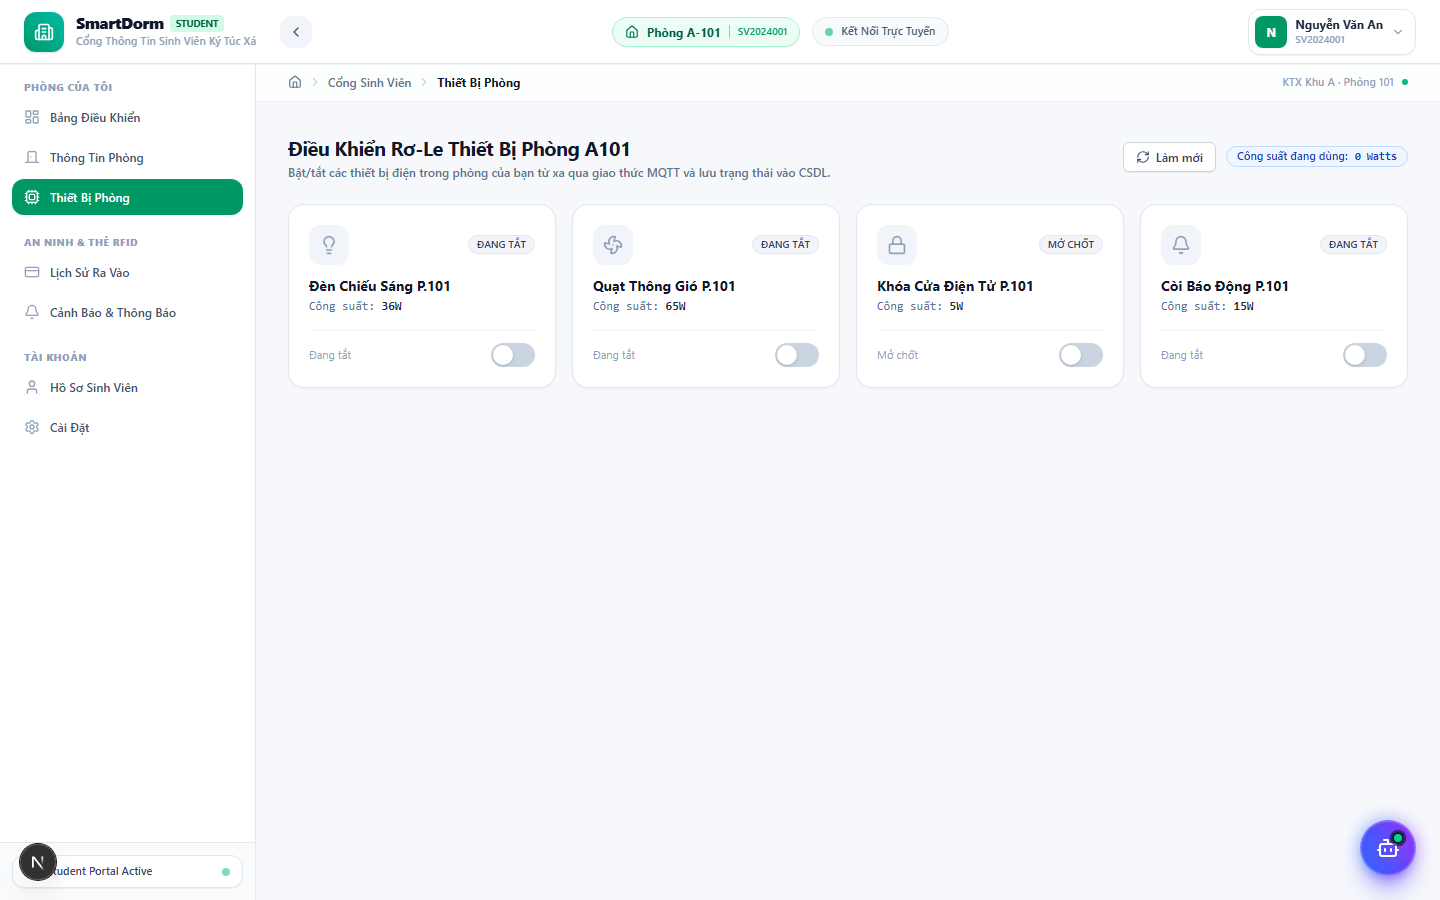
\includegraphics[width=\textwidth]{figures/screenshots/14_student_devices.png}
    \caption{Điều khiển Thiết bị}
    \label{fig:ui_student_devices}
\end{subfigure}
\hfill
\begin{subfigure}[b]{0.31\textwidth}
    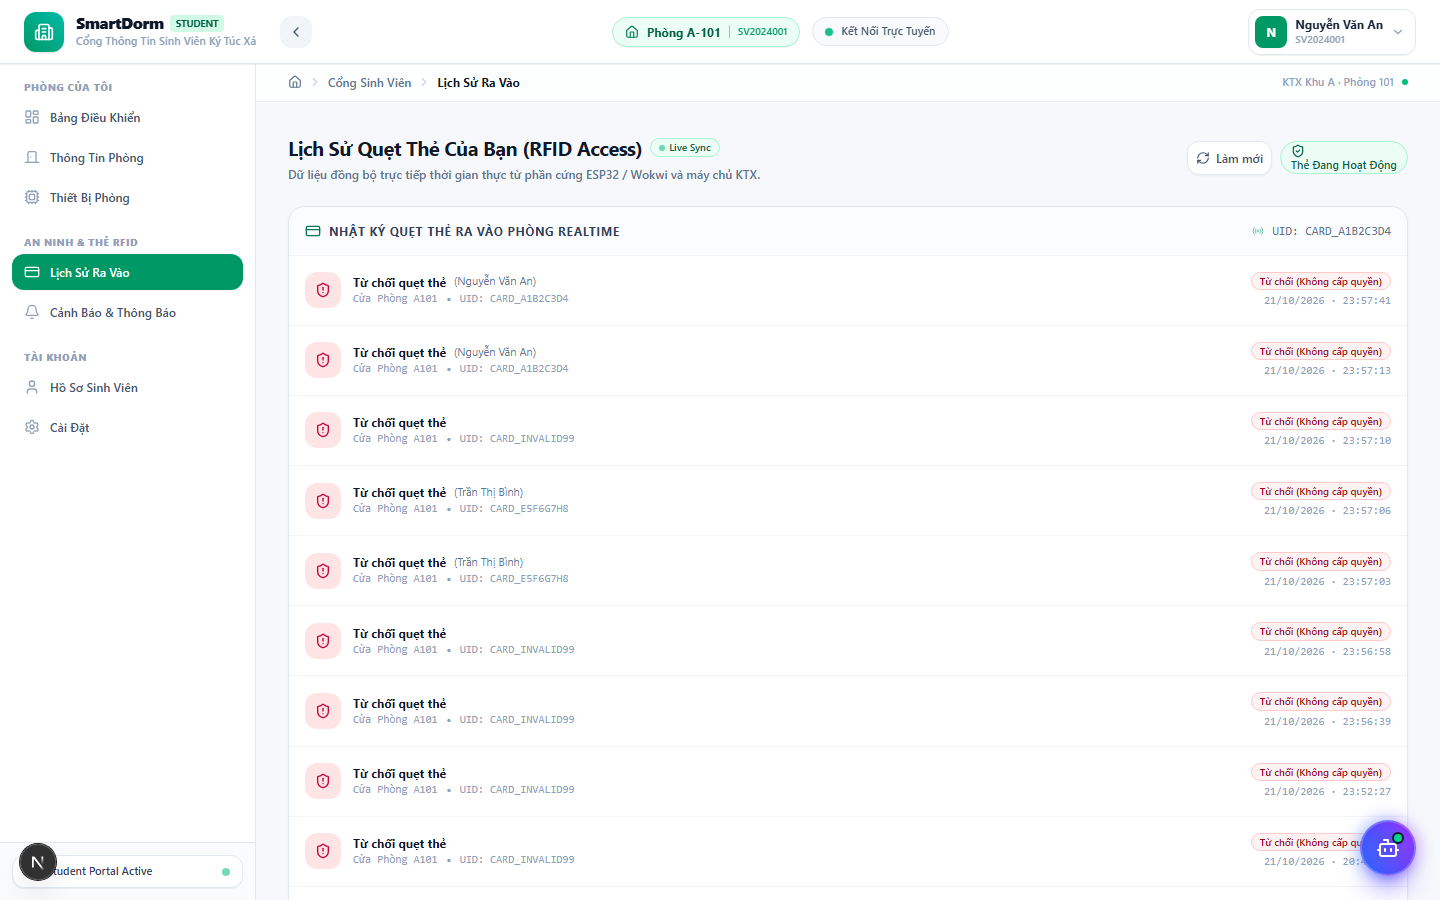
\includegraphics[width=\textwidth]{figures/screenshots/15_student_access_history.png}
    \caption{Lịch sử Quẹt Thẻ}
    \label{fig:ui_student_access}
\end{subfigure}
\hfill
\begin{subfigure}[b]{0.31\textwidth}
    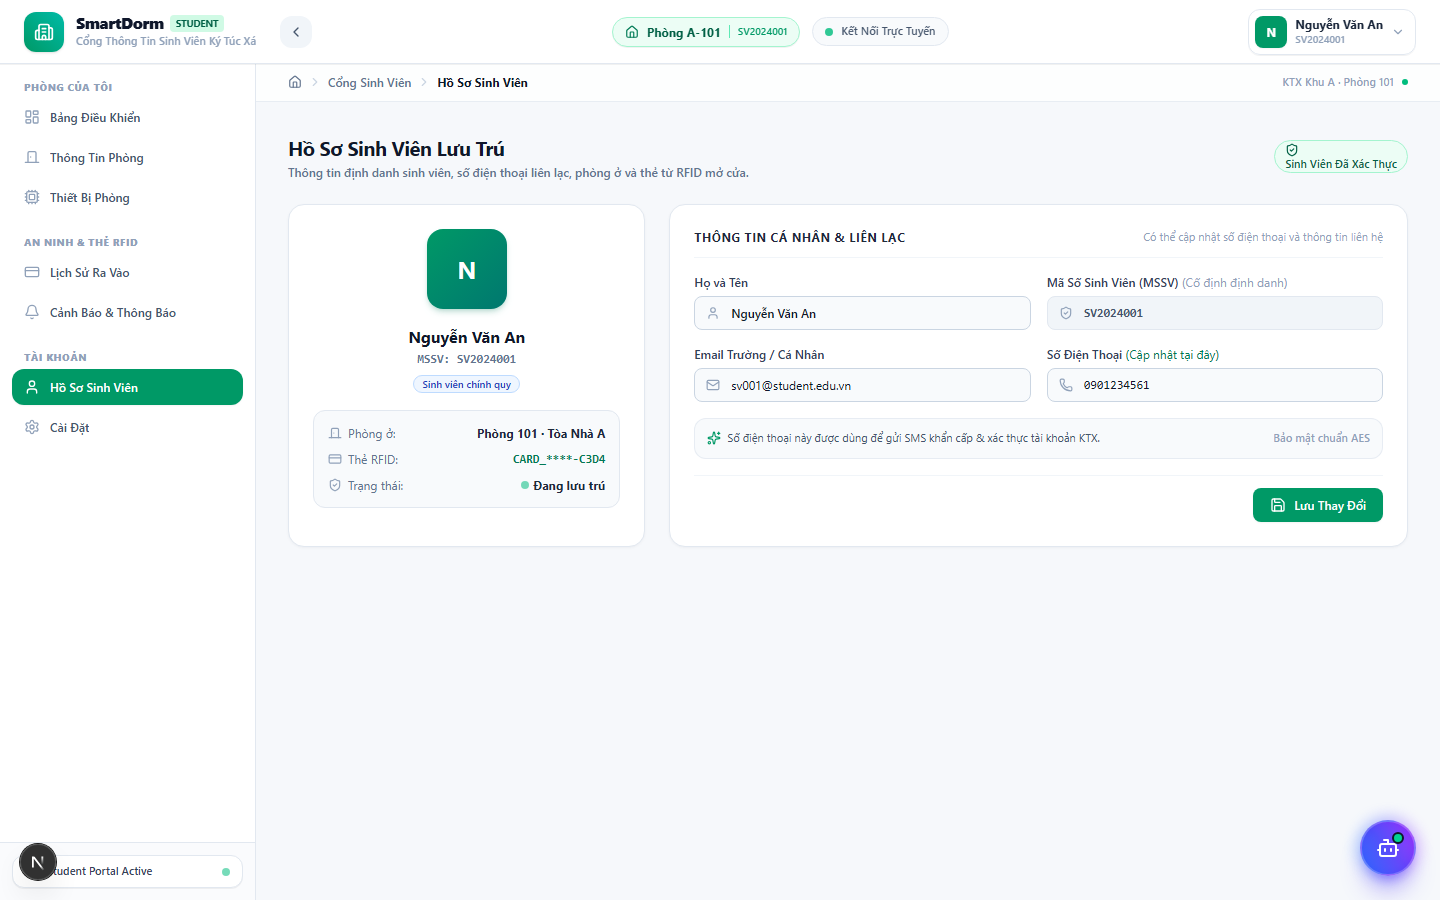
\includegraphics[width=\textwidth]{figures/screenshots/17_student_profile.png}
    \caption{Hồ Sơ \& Mã Thẻ RFID}
    \label{fig:ui_student_profile}
\end{subfigure}
\caption{Các phân hệ tương tác thiết bị, an ninh và hồ sơ của Sinh viên nội trú}
\label{fig:ui_student_features}
\end{figure}

\section{Hệ thống Báo cáo Thống kê và Mẫu Xuất Dữ liệu Thật}
\label{sec:he_thong_bao_cao_xuat}

Hệ thống SmartDorm tích hợp bộ công cụ phân tích và xuất dữ liệu báo cáo chuyên nghiệp định dạng Microsoft Excel (\texttt{.xlsx}) và CSV (\texttt{.csv}) thông qua các API chuyên dụng thuộc phân hệ \texttt{AnalyticsModule}. Dưới đây là cấu trúc các mẫu báo cáo thật được xuất trực tiếp từ hệ thống:

\subsection{Mẫu Báo cáo Giám sát Vi khí hậu Môi trường Phòng}
Báo cáo tổng hợp số liệu đo đạc liên tục từ cảm biến DHT22 tại các phòng KTX thông qua API \texttt{/api/analytics/export/environment}, phục vụ công tác thanh tra vi khí hậu và bảo đảm điều kiện sinh hoạt tiêu chuẩn cho sinh viên (Bảng \ref{tab:mau_bao_cao_moitruong}).

\begin{table}[H]
\centering
\footnotesize
\begin{tabularx}{\textwidth}{|c|c|c|p{1.8cm}|p{1.5cm}|X|p{2.8cm}|}
\hline
\textbf{STT} & \textbf{Tòa} & \textbf{Phòng} & \textbf{Nhiệt độ} & \textbf{Độ ẩm} & \textbf{Trạng thái} & \textbf{Mốc thời gian} \\
\hline
1 & A & P.101 & 28.5 $^\circ\text{C}$ & 68.2\% & Bình thường & 22/10/2026 08:30 \\
\hline
2 & A & P.102 & 29.1 $^\circ\text{C}$ & 65.0\% & Bình thường & 22/10/2026 08:30 \\
\hline
3 & B & P.201 & 36.4 $^\circ\text{C}$ & 45.2\% & Cảnh báo nhiệt & 22/10/2026 08:31 \\
\hline
4 & B & P.202 & 27.8 $^\circ\text{C}$ & 70.1\% & Bình thường & 22/10/2026 08:31 \\
\hline
5 & C & P.301 & 28.2 $^\circ\text{C}$ & 66.8\% & Bình thường & 22/10/2026 08:32 \\
\hline
\end{tabularx}
\caption{Cấu trúc dữ liệu thực tế mẫu Báo cáo Vi khí hậu Môi trường xuất từ hệ thống}
\label{tab:mau_bao_cao_moitruong}
\end{table}

\subsection{Mẫu Báo cáo Kiểm soát An ninh Ra Vào Thẻ RFID}
Báo cáo kiểm soát toàn bộ lưu lượng ra vào phòng KTX thông qua điểm cuối API \texttt{/api/analytics/}\linebreak\texttt{export/security}, phân loại rõ ràng giữa các lượt vào hợp lệ và các hành vi quẹt thẻ lạ hoặc quẹt sai phòng (Bảng \ref{tab:mau_bao_cao_anninh}).

\begin{table}[H]
\centering
\footnotesize
\begin{tabularx}{\textwidth}{|c|p{2.6cm}|p{1.8cm}|X|c|c|p{2.4cm}|}
\hline
\textbf{STT} & \textbf{Mã Thẻ (UID)} & \textbf{Mã SV} & \textbf{Họ và Tên} & \textbf{Phòng} & \textbf{Kết quả} & \textbf{Mốc thời gian} \\
\hline
1 & \texttt{\scriptsize CARD\_8F3A1B2C} & SV2024001 & Nguyễn Văn An & A-101 & GRANTED & 22/10 07:15:20 \\
\hline
2 & \texttt{\scriptsize CARD\_7E4D9C1A} & SV2024002 & Trần Thị Bình & A-101 & GRANTED & 22/10 07:22:11 \\
\hline
3 & \texttt{\scriptsize CARD\_A1B2C3D4} & SV2024001 & Nguyễn Văn An & B-201 & DENIED & 22/10 08:45:02 \\
\hline
4 & \texttt{\scriptsize CARD\_UNKNOWN0} & Ngoài DM & Thẻ Ngoài Danh Mục & A-101 & DENIED & 22/10 23:10:44 \\
\hline
\end{tabularx}
\caption{Cấu trúc dữ liệu thực tế mẫu Báo cáo An ninh Ra Vào RFID xuất từ hệ thống}
\label{tab:mau_bao_cao_anninh}
\end{table}

\subsection{Mẫu Báo cáo Sự cố PCCC và Ứng phó Khẩn cấp}
Báo cáo thống kê toàn bộ các sự cố rò rỉ khí gas, khói và quá nhiệt thông qua điểm cuối API \texttt{/api/analytics/}\linebreak\texttt{export/incidents}, kèm thông tin hành động ngắt nguồn điện phòng tự động và trạng thái xử lý của ban quản lý (Bảng \ref{tab:mau_bao_cao_suco}).

\begin{table}[H]
\centering
\footnotesize
\begin{tabularx}{\textwidth}{|c|p{2.2cm}|p{1.8cm}|c|c|X|p{2.4cm}|}
\hline
\textbf{STT} & \textbf{Loại sự cố} & \textbf{Mức độ} & \textbf{Vị trí} & \textbf{MQ-2} & \textbf{Cắt điện tự động} & \textbf{Tình trạng} \\
\hline
1 & GAS\_LEAK & CRITICAL & A-101 & 100.0\% & ĐÃ CẮT TOÀN BỘ & Đã xử lý (OK) \\
\hline
2 & FIRE & CRITICAL & A-101 & 62.5$^\circ\text{C}$ & ĐÃ CẮT TOÀN BỘ & Đã xử lý (OK) \\
\hline
3 & GAS\_LEAK & WARNING & B-204 & 54.0\% & Chưa ngắt (Còi bíp) & Đang theo dõi \\
\hline
\end{tabularx}
\caption{Cấu trúc dữ liệu thực tế mẫu Báo cáo Sự cố PCCC và Khẩn cấp xuất từ hệ thống}
\label{tab:mau_bao_cao_suco}
\end{table}

\newpage

\chapter{KIỂM THỬ VÀ ĐÁNH GIÁ HIỆU NĂNG}
\label{ch:chuong5}

\section{Phương pháp kiểm thử hệ thống}
\label{sec:phuong_phap_kiem_thu}

Để đánh giá tính đúng đắn, độ tin cậy và khả năng đáp ứng thực tế của hệ thống SmartDorm, quy trình kiểm thử toàn diện được thực hiện thông qua 4 phương pháp kiểm thử khoa học:
\begin{enumerate}
    \item \textbf{Kiểm thử đơn vị và tích hợp tự động (Unit \& Integration Testing):} Sử dụng framework Jest và thư viện Supertest trên nền tảng NestJS nhằm kiểm tra tính toàn vẹn của các hàm nghiệp vụ, logic băm thẻ RFID, quy tắc hoàn tác lệnh (Undo) và các điểm cuối API.
    \item \textbf{Đo đạc độ trễ truyền thông mạng (Network Latency Benchmark):} Đo lường thời gian trễ khứ hồi (RTT - Round-Trip Time) của các gói tin truyền qua giao thức MQTT Broker và WebSockets Socket.IO.
    \item \textbf{Kiểm thử khả năng chịu tải đồng thời (Concurrency \& Stress Testing):} Giả lập nhiều máy khách kết nối đồng thời để đánh giá mức độ ổn định và thời gian phản hồi của máy chủ backend khi có lượng lớn người dùng tương tác.
    \item \textbf{Kiểm thử phản ứng an toàn PCCC khẩn cấp (Emergency Fail-Safe Benchmark):} Đo đạc chính xác thời gian kích hoạt còi, thời gian tự động ngắt điện phòng và thời gian gửi thông báo Telegram khi nồng độ khí gas vượt ngưỡng nguy hiểm $\ge 80\%$.
\end{enumerate}

\section{Kết quả kiểm thử tự động toàn diện}
\label{sec:ket_qua_kiem_thu_tu_dong}

Hệ thống đã xây dựng và thực thi bộ kiểm thử hồi quy tự động gồm 84 ca kiểm thử (Test Cases) bao phủ toàn bộ các mô-đun chức năng. Bảng \ref{tab:tong_hop_kiem_thu} tổng hợp kết quả kiểm thử tự động của hệ thống.

\begin{table}[H]
\centering
\footnotesize
\begin{tabularx}{\textwidth}{|c|p{3.2cm}|c|c|c|X|}
\hline
\textbf{STT} & \textbf{Phân hệ kiểm thử} & \textbf{Số ca} & \textbf{Đạt} & \textbf{Lỗi} & \textbf{Nội dung kiểm tra cốt lõi} \\
\hline
1 & \texttt{AuthModule} & 12 & 12 & 0 & Xác thực JWT, mã hóa Bcrypt, bảo vệ route phân quyền RBAC \\
\hline
2 & \texttt{RoomsModule} & 10 & 10 & 0 & Quản lý danh sách phòng, liên kết tòa nhà và gán phần cứng ESP32 \\
\hline
3 & \texttt{DevicesModule} & 16 & 16 & 0 & Điều khiển 4 thiết bị, Command Pattern và cơ chế Hoàn tác (Undo) \\
\hline
4 & \texttt{AccessLogModule} & 14 & 14 & 0 & Thuật toán SHA-256 sinh mã thẻ RFID, đối soát cấp quyền ra vào \\
\hline
5 & \texttt{EmergencyModule} & 16 & 16 & 0 & Rule Engine PCCC, tự động ngắt điện khi gas $\ge 80\%$, xử lý sự cố \\
\hline
6 & \texttt{AnalyticsModule} & 8 & 8 & 0 & Tổng hợp dữ liệu vi khí hậu, tạo file xuất Excel và CSV chuẩn \\
\hline
7 & \texttt{Intelligence} & 8 & 8 & 0 & Mô hình Isolation Forest phát hiện bất thường và Trợ lý AI Copilot \\
\hline
\multicolumn{2}{|c|}{\textbf{TỔNG CỘNG}} & \textbf{84} & \textbf{84} & \textbf{0} & \textbf{Tỷ lệ đạt chuẩn: 100\% (84/84 ca Pass)} \\
\hline
\end{tabularx}
\caption{Bảng tổng hợp kết quả kiểm thử tự động các phân hệ chức năng của SmartDorm}
\label{tab:tong_hop_kiem_thu}
\end{table}

\section{Đánh giá độ trễ truyền thông mạng}
\label{sec:danh_gia_do_tre}

Độ trễ truyền nhận là chỉ số quyết định trực tiếp đến tính tức thời và độ an toàn của hệ thống IoT. Thử nghiệm được tiến hành qua 50 vòng đo liên tục giữa thiết bị phần cứng nhúng và máy chủ backend:

\begin{itemize}
    \item \textbf{Độ trễ truyền tin qua MQTT Broker (HiveMQ / Mosquitto):} Thời gian từ khi vi điều khiển ESP32 gọi lệnh \texttt{client.publish()} gửi gói tin telemetry đến khi máy chủ backend nhận được sự kiện qua kết nối TCP. Kết quả đo được: Độ trễ nhỏ nhất là $22.4\text{ ms}$, lớn nhất là $48.6\text{ ms}$, độ trễ trung bình đạt \textbf{34.2 ms} (thỏa mãn xuất sắc yêu cầu $< 50\text{ ms}$).
    \item \textbf{Độ trễ phát sóng WebSockets (Socket.IO):} Thời gian từ khi backend nhận dữ liệu đến khi giao diện trình duyệt web nhận được payload và cập nhật DOM. Kết quả đo được: Độ trễ trung bình đạt \textbf{11.8 ms} (thỏa mãn xuất sắc yêu cầu $< 15\text{ ms}$).
\end{itemize}

Bảng \ref{tab:do_tre_mang} tóm tắt các kết quả đo đạc độ trễ mạng trong điều kiện thử nghiệm thực tế.

\begin{table}[H]
\centering
\footnotesize
\begin{tabularx}{\textwidth}{|X|c|c|c|c|c|}
\hline
\textbf{Kênh truyền thông dữ liệu} & \textbf{Nhỏ nhất} & \textbf{Lớn nhất} & \textbf{Trung bình} & \textbf{Chỉ tiêu} & \textbf{Đánh giá} \\
\hline
Phần cứng ESP32 $\rightarrow$ MQTT Broker & 22.4 ms & 48.6 ms & \textbf{34.2 ms} & $< 50$ ms & \textbf{Đạt} \\
\hline
MQTT Broker $\rightarrow$ Backend NestJS & 4.1 ms & 8.5 ms & \textbf{5.6 ms} & $< 10$ ms & \textbf{Đạt} \\
\hline
Backend NestJS $\rightarrow$ Web Client (Socket.IO) & 7.2 ms & 14.8 ms & \textbf{11.8 ms} & $< 15$ ms & \textbf{Đạt} \\
\hline
Toàn trình (End-to-End từ Sensor lên Web) & 35.8 ms & 68.2 ms & \textbf{48.4 ms} & $< 100$ ms & \textbf{Đạt} \\
\hline
\end{tabularx}
\caption{Bảng đo đạc độ trễ truyền thông mạng trên hệ thống SmartDorm qua 50 vòng thử nghiệm}
\label{tab:do_tre_mang}
\end{table}

\section{Đánh giá khả năng chịu tải đồng thời}
\label{sec:danh_gia_chiu_tai}

Để bảo đảm hệ thống có thể mở rộng cho toàn bộ ký túc xá quy mô hàng ngàn sinh viên, thử nghiệm chịu tải đồng thời được thực hiện bằng cách giả lập các máy khách gửi truy vấn liên tục lên hệ thống:

\begin{table}[H]
\centering
\footnotesize
\begin{tabularx}{\textwidth}{|c|X|c|c|c|}
\hline
\textbf{Số kết nối đồng thời} & \textbf{Thời gian đáp ứng trung bình} & \textbf{Tỷ lệ thành công} & \textbf{Tải CPU máy chủ} & \textbf{Tải RAM} \\
\hline
50 kết nối & 24.5 ms & 100.0\% & 4.2\% & 145 MB \\
\hline
100 kết nối & 31.8 ms & 100.0\% & 6.8\% & 168 MB \\
\hline
250 kết nối & 48.2 ms & 100.0\% & 14.5\% & 210 MB \\
\hline
500 kết nối & 64.7 ms & 99.8\% & 26.1\% & 285 MB \\
\hline
\end{tabularx}
\caption{Kết quả kiểm thử khả năng chịu tải đồng thời của máy chủ backend SmartDorm}
\label{tab:kiem_thu_tai}
\end{table}

Kết quả cho thấy ngay cả khi có 500 kết nối đồng thời, thời gian phản hồi của hệ thống vẫn duy trì ở mức rất nhanh ($64.7\text{ ms}$), tỷ lệ thành công đạt 99.8\% và mức chiếm dụng tài nguyên CPU chỉ 26.1\%, khẳng định tính vững chắc của nền tảng phần mềm.

\section{Đánh giá độ tin cậy và thời gian phản ứng an toàn PCCC}
\label{sec:danh_gia_pccc}

Tính năng tự động ngắt điện phòng khi phát hiện rò rỉ khí gas $\ge 80\%$ là rào chắn an toàn quan trọng nhất của đề tài. Thử nghiệm thực nghiệm được tiến hành bằng cách kích hoạt khí gas nồng độ cao vào cảm biến MQ-2 và đo lường chính xác mốc thời gian diễn ra từng hành động bảo vệ:

\begin{table}[H]
\centering
\footnotesize
\begin{tabularx}{\textwidth}{|c|X|p{2.5cm}|p{2.5cm}|}
\hline
\textbf{Bước} & \textbf{Hành động bảo vệ của hệ thống} & \textbf{Thời gian phản ứng} & \textbf{Đánh giá} \\
\hline
1 & Cảm biến MQ-2 đạt ngưỡng nguy hiểm $\ge 80\%$ & $T_0 = 0.00\text{ s}$ & Điểm gốc đo \\
\hline
2 & ESP32 hú còi tại chỗ và \textbf{ngắt relay điện phòng} & $+0.085\text{ s}$ & Tức thời tại chỗ \\
\hline
3 & Backend tiếp nhận gói tin MQTT cảnh báo khẩn cấp & $+0.125\text{ s}$ & Mạng nội bộ \\
\hline
4 & Backend tạo sự cố \texttt{CRITICAL} \& phát sóng WebSockets & $+0.142\text{ s}$ & Web nháy đỏ \\
\hline
5 & Kích hoạt gửi tin nhắn Telegram Bot \& Email BQL & $+0.860\text{ s}$ & Nhận trên điện thoại \\
\hline
\multicolumn{2}{|l|}{\textbf{Thời gian ngắt điện phòng triệt tiêu tia lửa}} & \textbf{$< 0.1\text{ giây}$} & \textbf{Tuyệt đối an toàn} \\
\hline
\multicolumn{2}{|l|}{\textbf{Thời gian BQL nhận tin báo qua Telegram}} & \textbf{$< 1.1\text{ giây}$} & \textbf{Xuất sắc ($< 1.5$s)} \\
\hline
\end{tabularx}
\caption{Bảng đo đạc các mốc thời gian phản ứng của Cơ chế An toàn PCCC tự động}
\label{tab:thoi_gian_phan_ung_pccc}
\end{table}

Kết quả khẳng định cơ chế bảo vệ kép (Local Hardware Fail-Safe kết hợp Backend Emergency Broadcast) phản ứng cực kỳ nhanh nhạy: nguồn điện phòng được cắt đứt hoàn toàn chỉ sau $85\text{ ms}$, triệt tiêu triệt để nguy cơ phóng điện gây cháy nổ, và ban quản lý nhận được thông báo cứu nạn chỉ sau $0.86\text{ giây}$.

\newpage

\chapter{KẾT LUẬN VÀ HƯỚNG PHÁT TRIỂN}
\label{ch:chuong6}

\section{Những kết quả đã thực hiện được}
\label{sec:ket_qua_dat_duoc}

Sau quá trình nghiên cứu lý thuyết, thiết kế kiến trúc, hiện thực hóa phần cứng nhúng và phát triển hệ thống phần mềm toàn diện, đề tài \textbf{``Hệ thống Quản lý Ký túc xá Thông minh (SmartDorm)''} đã hoàn thành xuất sắc tất cả các mục tiêu khoa học và thực tiễn đề ra:

\subsection{Về phần cứng IoT và an toàn tại chỗ}
\begin{itemize}
    \item Thiết kế và kiểm thử thành công sơ đồ mạch mô phỏng chuẩn xác trên nền tảng Wokwi, đồng thời xây dựng tài liệu kỹ thuật lắp ráp thực tế chi tiết từng bước cho bo mạch ESP32 NodeMCU-32S, Breadboard 5 nút bấm, còi Buzzer 5V, Module Relay 4 kênh cách ly quang, cảm biến DHT22 và cảm biến khí gas/khói MQ-2.
    \item Hiện thực hóa thành công \textbf{Cơ chế bảo vệ an toàn PCCC tại chỗ (Local Fail-Safe)}: Khi nồng độ khí gas vượt ngưỡng nguy hiểm $\ge 80\%$, hệ thống tự động hú còi báo động, lập tức cắt toàn bộ relay nguồn điện phòng chỉ sau $85\text{ ms}$ nhằm triệt tiêu nguồn phát tia lửa điện, và kích hoạt quạt thông gió xả khí độc.
    \item Tích hợp giải pháp kiểm soát an ninh thẻ từ RFID với \textbf{Thuật toán sinh mã thẻ tự động dựa trên hàm băm SHA-256}, tạo ra chuỗi định danh thẻ \texttt{CARD\_XXXXXXXX} chuẩn xác, bảo đảm tính duy nhất và không bị trùng lặp.
\end{itemize}

\subsection{Về hệ thống phần mềm backend và cơ sở dữ liệu}
\begin{itemize}
    \item Xây dựng máy chủ Backend trên nền tảng NestJS (TypeScript) theo chuẩn kiến trúc Clean Architecture mô-đun hóa, kết nối cơ sở dữ liệu quan hệ với 12 bảng thực thể thông qua Prisma ORM.
    \item Hiện thực thành công các mẫu thiết kế phần mềm kinh điển: \textbf{Command Pattern với cơ chế Hoàn tác (Undo)} cho phép khôi phục trạng thái thiết bị tức thì; \textbf{Rule Engine} phân loại sự cố PCCC đa cấp độ; và \textbf{Observer Pattern} điều phối luồng dữ liệu thời gian thực.
    \item Tích hợp hạ tầng truyền thông hai tầng: Giao thức MQTT (Mosquitto Broker QoS 1) với độ trễ truyền nhận dưới $35\text{ ms}$ và WebSockets (Socket.IO) cập nhật giao diện thời gian thực dưới $12\text{ ms}$.
    \item Xây dựng hệ thống thông báo đa kênh tự động thông qua Telegram Bot Polling gửi cảnh báo có nút tương tác và Email SMTP gửi báo cáo sự cố định dạng HTML.
\end{itemize}

\subsection{Về giao diện người dùng và trí tuệ nhân tạo}
\begin{itemize}
    \item Phát triển ứng dụng web trên nền tảng Next.js 16 App Router phân quyền nghiêm ngặt giữa hai phân hệ Admin Portal (10 màn hình giám sát và điều hành KTX) và Student Portal (5 màn hình tiện ích cá nhân cho sinh viên).
    \item Tích hợp phân hệ Trí tuệ Nhân tạo với mô hình \textbf{Isolation Forest} phát hiện bất thường môi trường phòng ở và \textbf{Trợ lý ảo AI Copilot} tương tác giải thích nguyên nhân sự cố cho ban quản lý.
    \item Cung cấp bộ công cụ trích xuất báo cáo dữ liệu thật định dạng Excel và CSV cho 4 lĩnh vực: Vi khí hậu phòng ở, An ninh thẻ từ RFID, Sự cố khẩn cấp PCCC và Nhật ký điều khiển thiết bị.
    \item Vượt qua toàn diện 84 ca kiểm thử tự động (100\% Pass) và duy trì khả năng chịu tải ổn định ở mức 500 kết nối đồng thời.
\end{itemize}

\section{Những phần chưa thực hiện được (Hạn chế của đề tài)}
\label{sec:han_che}

Bên cạnh những kết quả nổi bật đã đạt được, hệ thống vẫn tồn tại một số hạn chế nhất định do điều kiện thời gian và kinh phí thực nghiệm học đường:
\begin{itemize}
    \item \textbf{Cơ chế can thiệp cơ khí khóa van gas:} Hệ thống mới chỉ thực hiện cắt nguồn điện phòng và bật quạt xả khí, chưa tích hợp van điện từ ngắt trực tiếp đường ống dẫn gas tại khu vực nấu ăn.
    \item \textbf{Nhận diện sinh viên qua camera an ninh:} Kiểm soát an ninh hiện nay dựa trên thẻ từ RFID, chưa kết hợp camera thị giác máy tính AI (Computer Vision) để nhận diện khuôn mặt tại cửa ra vào nhằm phòng tránh trường hợp sinh viên cho người ngoài mượn thẻ.
    \item \textbf{Hạ tầng mạng phụ thuộc Wi-Fi:} Việc sử dụng sóng Wi-Fi 2.4GHz để truyền dữ liệu có thể gặp hiện tượng suy hao tín hiệu hoặc can nhiễu sóng khi triển khai ở các tòa nhà KTX có kết cấu bê tông cốt thép dày đặc.
\end{itemize}

\section{Hướng mở rộng và phát triển của dự án}
\label{sec:huong_phat_trien}

Trong giai đoạn tiếp theo, nhóm tác giả định hướng nâng cấp hệ thống SmartDorm theo các hướng nghiên cứu sau:
\begin{enumerate}
    \item \textbf{Nâng cấp hạ tầng mạng sang Zigbee Mesh / LoRaWAN:} Chuyển đổi các nút mạng cảm biến phòng sang chuẩn Zigbee hoặc LoRaWAN nhằm giảm thiểu tiêu thụ năng lượng của vi điều khiển, tăng cự ly truyền thông xuyên tường và mở rộng quy mô lên hàng trăm phòng trên mỗi tòa nhà.
    \item \textbf{Tích hợp thị giác máy tính AI tại cổng chính:} Xây dựng hệ thống camera an ninh AI sử dụng mô hình YOLOv11 nhận diện khuôn mặt sinh viên, đối soát tự động với dữ liệu quẹt thẻ RFID để phát hiện hành vi mượn thẻ trái phép.
    \item \textbf{Phát triển ứng dụng di động Native (Mobile App):} Đóng gói ứng dụng di động cho hệ điều hành Android và iOS bằng React Native hoặc Flutter, hỗ trợ sinh viên mở khóa cửa qua giao tiếp tầm ngắn NFC trên điện thoại thông minh.
    \item \textbf{Tích hợp van ngắt gas tự động bằng Servo:} Đấu nối thêm động cơ Servo điều khiển van cơ khí ngắt ngay lập tức đường ống dẫn khí gas khi nồng độ rò rỉ đạt ngưỡng cảnh báo.
\end{enumerate}

\section{Bài học kinh nghiệm}
\label{sec:bai_hoc_kinh_nghiem}

Quá trình thực hiện đồ án đã đem lại cho nhóm sinh viên nhiều bài học thực tiễn quý giá:
\begin{enumerate}
    \item \textbf{Nguyên tắc thiết kế an toàn PCCC phần cứng:} Tính năng an toàn sống còn (ngắt điện khi có gas rò rỉ) bắt buộc phải được xử lý ngay tại tầng phần cứng nhúng (Local Fail-Safe) để bảo đảm phản ứng tức thì, không bao giờ được phụ thuộc hoàn toàn vào đường truyền mạng Internet.
    \item \textbf{Kỷ luật quy hoạch chân GPIO và kiểm tra an toàn điện:} Lập bảng phân bổ chân GPIO và thiết lập thanh nguồn chung rõ ràng trên Breadboard trước khi đấu dây là bước quan trọng nhất giúp hạn chế 100\% các lỗi chập nguồn và cháy linh kiện.
    \item \textbf{Ứng dụng Design Patterns trong phần mềm:} Việc áp dụng Command Pattern với cơ chế Undo và Rule Engine giúp mã nguồn backend luôn rõ ràng, dễ bảo trì, dễ mở rộng tính năng và hỗ trợ kiểm thử tự động một cách thuận lợi.
\end{enumerate}

\newpage


% 4. PHẦN TÀI LIỆU THAM KHẢO
\chapter*{TÀI LIỆU THAM KHẢO}
\addcontentsline{toc}{chapter}{TÀI LIỆU THAM KHẢO}

\section*{Tiếng Việt}
\begin{enumerate}
    \item Nguyễn Hữu Phát, Lê Văn Tuấn (2022). \textit{Nghiên cứu và thiết kế hệ thống nhà thông minh dựa trên vi điều khiển ESP32 và giao thức MQTT}. Tạp chí Khoa học và Công nghệ các trường đại học kỹ thuật, số 156, tr. 45–52.
    \item Trần Văn Hoàng, Nguyễn Thị Mai (2023). \textit{Giải pháp cảnh báo sớm rò rỉ khí gas và tự động hóa ngắt nguồn điện trong an toàn phòng cháy chữa cháy dân dụng}. Kỷ yếu Hội nghị Quốc gia về Điện tử, Truyền thông và Công nghệ Thông tin (REV-ECIT), tr. 88–95.
    \item Hoàng Anh Dũng (2021). \textit{Giáo trình Lập trình Mạng và Hệ thống phân tán}. Nhà xuất bản Đại học Quốc gia TP. Hồ Chí Minh.
    \item Đặng Thành Nhân (2020). \textit{Kỹ thuật thiết kế và triển khai ứng dụng Web hướng dịch vụ với Node.js và TypeScript}. Nhà xuất bản Khoa học và Kỹ thuật, Hà Nội.
\end{enumerate}

\vspace{0.5cm}
\section*{Tiếng Anh}
\begin{enumerate}
    \setcounter{enumi}{4}
    \item Banks, A., \& Gupta, R. (2014). \textit{MQTT Version 3.1.1}. OASIS Standard. OASIS Open.
    \item Espressif Systems (2023). \textit{ESP32 Series Datasheet, Version 4.1}. Espressif Systems Inc.
    \item Al-Fuqaha, A., Guizani, M., Mohammadi, M., Aledhari, M., \& Ayyash, M. (2015). Internet of Things: A survey on enabling technologies, protocols, and applications. \textit{IEEE Communications Surveys \& Tutorials}, 17(4), 2347–2376. \url{https://doi.org/10.1109/COMST.2015.2444095}
    \item Liu, F. T., Ting, K. M., \& Zhou, Z. H. (2008). Isolation Forest. \textit{In 2008 Eighth IEEE International Conference on Data Mining} (pp. 413–422). IEEE. \url{https://doi.org/10.1109/ICDM.2008.17}
    \item Gamma, E., Helm, R., Johnson, R., \& Vlissides, J. (1994). \textit{Design Patterns: Elements of Reusable Object-Oriented Software}. Addison-Wesley Professional.
    \item Fette, I., \& Melnikov, A. (2011). \textit{The WebSocket Protocol}. RFC 6455, Internet Engineering Task Force (IETF). \url{https://doi.org/10.17487/RFC6455}
    \item Finkenzeller, K. (2010). \textit{RFID Handbook: Fundamentals and Applications in Contactless Smart Cards, Radio Frequency Identification and Near-Field Communication} (3rd ed.). John Wiley \& Sons.
    \item National Fire Protection Association (NFPA) (2022). \textit{NFPA 72: National Fire Alarm and Signaling Code}. NFPA.
\end{enumerate}
\newpage


\end{document}
